\documentclass[a4paper, 12pt, twoside]{report}
\usepackage[T1]{fontenc}
\usepackage[utf8]{inputenc}
\usepackage[italian]{babel}
\usepackage{geometry}
\usepackage{graphicx}
\usepackage{wrapfig2}
\usepackage{amsmath}
\usepackage{cancel} %semplificazione
\usepackage{amssymb}
\usepackage{amsthm} %teoremi e dimostrazioni e definizioni
\usepackage{gensymb} %simboli come ° = \degree  etc etc
\usepackage{cases}
\usepackage{subcaption}
\usepackage{hyperref}
\hypersetup{
	colorlinks=true,
	linkcolor=blue,    
	urlcolor=blue,
	%pdfpagemode=FullScreen,
}
\urlstyle{same}
\usepackage{color} % testo colorato
\raggedbottom
\setlength{\parindent}{0pt}
\usepackage{multirow}
\usepackage{booktabs} %tabelle scientifiche
\usepackage{listings} %importa i codici 
%%%%%%%%%%%%%%%%%%%%%%%%%%%%%%%%%%%%%%%%%%%% SIUNITX 
\usepackage{siunitx}

%%%%%%%%%%%%%%%%%%%%%%%%%%%%%%%%%%%%%%%%%%%% AMBIENTE TIKZ 
\usepackage{tikz} %disegni e mappe
\usetikzlibrary{patterns}
\usepackage{pgfplots}
\pgfplotsset{compat=1.15}
\usepackage{mathrsfs}
\usetikzlibrary{arrows,decorations.markings,arrows.meta, decorations.text}

\tikzset{immagine/.style={%
		above right, inner sep=0pt, outer sep=0pt},
	testo/.style={fill=white, align=center,
		fill opacity=0.6, text opacity=1, below,
		font=\sffamily\bfseries\footnotesize}}



%%%%%%%%%%%%%%%%%%%%%%%%%%%%%%%%%%%%%%%%%%%%%%%%%%%%%%%%% NUOVI COMANDI
\newcommand{\ra}[1]{\renewcommand{\arraystretch}{#1}} %stretcho le tabelle

		
		
		\begin{document}
			\begin{titlepage}
				\begin{center}
					
					
\includegraphics[width=0.8\textwidth]{figures/unitus_marchio_2020_DEIM}
					
					\vspace{0.5cm}
					
					{\Large Corso di Laurea in Ingegneria Industriale}
					
					\vspace{0.5cm}
					
					{\Large Laboratorio di Misure Meccaniche e Termiche}
					
					\vspace{0.5cm}
					
					{\Large A.A 2022-2023}
					
					\vspace{1.5cm}
					
					\textbf{{\Huge Relazione Esercitazione 1}}
					
					\vspace{0.5cm}
					{\LARGE Sistemi del primo e secondo ordine}
					
					\vspace{1.5cm}
					
					\textbf{Andrea Marchegiani, Gruppo 3, mat. 810513}\\
					\href{mailto:andrea.marchegiani@studenti.unitus.it}{andrea.marchegiani@studenti.unitus.it} 
					
					
					\vfill
					
					
					
					24/10/2022
					
				\end{center}
			\end{titlepage}
			
			
			\setcounterpageref{secnumdepth}{0}	
			\tableofcontents 
			\newpage
		
		
		\section{Parte 1: Sistemi del primo ordine} 
		\subsection{Misura sperimentale della costante di tempo}
		Un sistema del primo ordine è caratterizzato da una risposta in frequenza definita da un solo parametro, la costante di tempo $\tau$. \newline
		
		In questa esperienza si calcolerà la costante di tempo attraverso il metodo grafico e quello analitico.  
		
		\paragraph{Metodo grafico o Metodo delle Sottotangenti} \mbox{} \\ 
		L'andamento nel tempo di un sistema del primo ordine è prevedibile attraverso una forma esponenziale.
		
		Se allo strumento è fornito un gradino decrescente, questo risponderà con un'esponenziale decrescente:
		\[y(t) = A_0e^{-t/\tau}\]
		Derivandola si ottiene:
		\[\dot{y}(t) = -{1\over\tau}A_0e^{-t/\tau}\]
		La derivata di una funzione è la retta tangente a tale funzione nel punto considerato.
		 
		Con riferimento alla figura sottostante, la tangente dell’angolo $\beta$ in $ x = 1 $ si trova geometricamente nel
		seguente modo:
 		\[a\sin(\beta) = c \hspace{1cm} a\cos(\beta) = b\]
		\[\tan(\beta) = {c\over b}\]
		Ma la stessa tangente si può calcolare come:
		\[ \dot{y}(0) = -{1\over\tau}A_0 \]
		Per cui: 
		\[{c\over b} = -{1\over\tau}A_0 \Leftrightarrow c=A_0\quad b = \tau \]
		
		Ad esempio se:
		\[y(t) = e^{-t} \Rightarrow b = \tau = 1\]
					
		\definecolor{ccqqqq}{rgb}{0.8,0.,0.}
		\definecolor{qqwuqq}{rgb}{0.,0.39215686274509803,0.}
		\begin{figure}[H]
			\centering				
	\subfloat{\scalebox{0.8}{\begin{tikzpicture}[line cap=round,line join=round,>=triangle 45]
			\begin{axis}[
				x=5cm,y=5cm,
				axis lines=middle,
				%					ymajorgrids=true,
				%					xmajorgrids=true,
				xmin=-0.18,
				xmax=1.85,
				ymin=0,
				ymax=1.45,
				ytick=\empty, xtick=\empty,
				xticklabels=\empty,yticklabels=\empty,extra x ticks={0,1}, extra y ticks={1},
				xlabel=$x$, ylabel=$y$]
				\clip(-0.2,-0.1) rectangle (1.8,1.4);
				%%%%%%%%%%%%%%%%%%%% ESPONENZIALE
				\draw[line width=2.pt,color=qqwuqq] (-0.2,1.2214027581601699) -- (-0.2,1.2214027581601699);
				\draw[line width=2.pt,color=qqwuqq] (-0.2,1.2214027581601699) -- (-0.195,1.2153109864897307);
				\draw[line width=2.pt,color=qqwuqq] (-0.195,1.2153109864897307) -- (-0.19,1.2092495976572515);
				\draw[line width=2.pt,color=qqwuqq] (-0.19,1.2092495976572515) -- (-0.185,1.2032184401276953);
				\draw[line width=2.pt,color=qqwuqq] (-0.185,1.2032184401276953) -- (-0.18,1.1972173631218102);
				\draw[line width=2.pt,color=qqwuqq] (-0.18,1.1972173631218102) -- (-0.175,1.191246216612358);
				\draw[line width=2.pt,color=qqwuqq] (-0.175,1.191246216612358) -- (-0.16999999999999998,1.1853048513203654);
				\draw[line width=2.pt,color=qqwuqq] (-0.16999999999999998,1.1853048513203654) -- (-0.16499999999999998,1.1793931187113906);
				\draw[line width=2.pt,color=qqwuqq] (-0.16499999999999998,1.1793931187113906) -- (-0.15999999999999998,1.1735108709918103);
				\draw[line width=2.pt,color=qqwuqq] (-0.15999999999999998,1.1735108709918103) -- (-0.15499999999999997,1.167657961105125);
				\draw[line width=2.pt,color=qqwuqq] (-0.15499999999999997,1.167657961105125) -- (-0.14999999999999997,1.161834242728283);
				\draw[line width=2.pt,color=qqwuqq] (-0.14999999999999997,1.161834242728283) -- (-0.14499999999999996,1.1560395702680215);
				\draw[line width=2.pt,color=qqwuqq] (-0.14499999999999996,1.1560395702680215) -- (-0.13999999999999996,1.1502737988572271);
				\draw[line width=2.pt,color=qqwuqq] (-0.13999999999999996,1.1502737988572271) -- (-0.13499999999999995,1.1445367843513143);
				\draw[line width=2.pt,color=qqwuqq] (-0.13499999999999995,1.1445367843513143) -- (-0.12999999999999995,1.1388283833246218);
				\draw[line width=2.pt,color=qqwuqq] (-0.12999999999999995,1.1388283833246218) -- (-0.12499999999999994,1.1331484530668263);
				\draw[line width=2.pt,color=qqwuqq] (-0.12499999999999994,1.1331484530668263) -- (-0.11999999999999994,1.1274968515793755);
				\draw[line width=2.pt,color=qqwuqq] (-0.11999999999999994,1.1274968515793755) -- (-0.11499999999999994,1.1218734375719384);
				\draw[line width=2.pt,color=qqwuqq] (-0.11499999999999994,1.1218734375719384) -- (-0.10999999999999993,1.1162780704588713);
				\draw[line width=2.pt,color=qqwuqq] (-0.10999999999999993,1.1162780704588713) -- (-0.10499999999999993,1.1107106103557052);
				\draw[line width=2.pt,color=qqwuqq] (-0.10499999999999993,1.1107106103557052) -- (-0.09999999999999992,1.1051709180756475);
				\draw[line width=2.pt,color=qqwuqq] (-0.09999999999999992,1.1051709180756475) -- (-0.09499999999999992,1.0996588551261028);
				\draw[line width=2.pt,color=qqwuqq] (-0.09499999999999992,1.0996588551261028) -- (-0.08999999999999991,1.0941742837052102);
				\draw[line width=2.pt,color=qqwuqq] (-0.08999999999999991,1.0941742837052102) -- (-0.08499999999999991,1.0887170666983985);
				\draw[line width=2.pt,color=qqwuqq] (-0.08499999999999991,1.0887170666983985) -- (-0.0799999999999999,1.0832870676749584);
				\draw[line width=2.pt,color=qqwuqq] (-0.0799999999999999,1.0832870676749584) -- (-0.0749999999999999,1.0778841508846315);
				\draw[line width=2.pt,color=qqwuqq] (-0.0749999999999999,1.0778841508846315) -- (-0.0699999999999999,1.0725081812542163);
				\draw[line width=2.pt,color=qqwuqq] (-0.0699999999999999,1.0725081812542163) -- (-0.06499999999999989,1.0671590243841924);
				\draw[line width=2.pt,color=qqwuqq] (-0.06499999999999989,1.0671590243841924) -- (-0.059999999999999894,1.0618365465453594);
				\draw[line width=2.pt,color=qqwuqq] (-0.059999999999999894,1.0618365465453594) -- (-0.054999999999999896,1.056540614675494);
				\draw[line width=2.pt,color=qqwuqq] (-0.054999999999999896,1.056540614675494) -- (-0.0499999999999999,1.051271096376024);
				\draw[line width=2.pt,color=qqwuqq] (-0.0499999999999999,1.051271096376024) -- (-0.0449999999999999,1.046027859908717);
				\draw[line width=2.pt,color=qqwuqq] (-0.0449999999999999,1.046027859908717) -- (-0.039999999999999904,1.0408107741923882);
				\draw[line width=2.pt,color=qqwuqq] (-0.039999999999999904,1.0408107741923882) -- (-0.034999999999999906,1.035619708799623);
				\draw[line width=2.pt,color=qqwuqq] (-0.034999999999999906,1.035619708799623) -- (-0.029999999999999905,1.0304545339535167);
				\draw[line width=2.pt,color=qqwuqq] (-0.029999999999999905,1.0304545339535167) -- (-0.024999999999999904,1.0253151205244286);
				\draw[line width=2.pt,color=qqwuqq] (-0.024999999999999904,1.0253151205244286) -- (-0.019999999999999903,1.0202013400267558);
				\draw[line width=2.pt,color=qqwuqq] (-0.019999999999999903,1.0202013400267558) -- (-0.014999999999999902,1.015113064615719);
				\draw[line width=2.pt,color=qqwuqq] (-0.014999999999999902,1.015113064615719) -- (-0.009999999999999901,1.010050167084168);
				\draw[line width=2.pt,color=qqwuqq] (-0.009999999999999901,1.010050167084168) -- (-0.004999999999999901,1.005012520859401);
				\draw[line width=2.pt,color=qqwuqq] (-0.004999999999999901,1.005012520859401) -- (0.0,0.9999999999999999);
				\draw[line width=2.pt,color=qqwuqq] (0.0,0.9999999999999999) -- (0.005000000000000099,0.9950124791926822);
				\draw[line width=2.pt,color=qqwuqq] (0.005000000000000099,0.9950124791926822) -- (0.010000000000000099,0.990049833749168);
				\draw[line width=2.pt,color=qqwuqq] (0.010000000000000099,0.990049833749168) -- (0.0150000000000001,0.9851119396030625);
				\draw[line width=2.pt,color=qqwuqq] (0.0150000000000001,0.9851119396030625) -- (0.0200000000000001,0.9801986733067553);
				\draw[line width=2.pt,color=qqwuqq] (0.0200000000000001,0.9801986733067553) -- (0.025000000000000102,0.9753099120283326);
				\draw[line width=2.pt,color=qqwuqq] (0.025000000000000102,0.9753099120283326) -- (0.030000000000000103,0.970445533548508);
				\draw[line width=2.pt,color=qqwuqq] (0.030000000000000103,0.970445533548508) -- (0.0350000000000001,0.9656054162575664);
				\draw[line width=2.pt,color=qqwuqq] (0.0350000000000001,0.9656054162575664) -- (0.0400000000000001,0.9607894391523231);
				\draw[line width=2.pt,color=qqwuqq] (0.0400000000000001,0.9607894391523231) -- (0.045000000000000095,0.9559974818330998);
				\draw[line width=2.pt,color=qqwuqq] (0.045000000000000095,0.9559974818330998) -- (0.05000000000000009,0.9512294245007139);
				\draw[line width=2.pt,color=qqwuqq] (0.05000000000000009,0.9512294245007139) -- (0.05500000000000009,0.9464851479534838);
				\draw[line width=2.pt,color=qqwuqq] (0.05500000000000009,0.9464851479534838) -- (0.06000000000000009,0.9417645335842486);
				\draw[line width=2.pt,color=qqwuqq] (0.06000000000000009,0.9417645335842486) -- (0.06500000000000009,0.9370674633774033);
				\draw[line width=2.pt,color=qqwuqq] (0.06500000000000009,0.9370674633774033) -- (0.07000000000000009,0.9323938199059482);
				\draw[line width=2.pt,color=qqwuqq] (0.07000000000000009,0.9323938199059482) -- (0.0750000000000001,0.9277434863285529);
				\draw[line width=2.pt,color=qqwuqq] (0.0750000000000001,0.9277434863285529) -- (0.0800000000000001,0.9231163463866356);
				\draw[line width=2.pt,color=qqwuqq] (0.0800000000000001,0.9231163463866356) -- (0.0850000000000001,0.9185122844014573);
				\draw[line width=2.pt,color=qqwuqq] (0.0850000000000001,0.9185122844014573) -- (0.09000000000000011,0.9139311852712281);
				\draw[line width=2.pt,color=qqwuqq] (0.09000000000000011,0.9139311852712281) -- (0.09500000000000011,0.9093729344682313);
				\draw[line width=2.pt,color=qqwuqq] (0.09500000000000011,0.9093729344682313) -- (0.10000000000000012,0.9048374180359595);
				\draw[line width=2.pt,color=qqwuqq] (0.10000000000000012,0.9048374180359595) -- (0.10500000000000012,0.9003245225862655);
				\draw[line width=2.pt,color=qqwuqq] (0.10500000000000012,0.9003245225862655) -- (0.11000000000000013,0.8958341352965281);
				\draw[line width=2.pt,color=qqwuqq] (0.11000000000000013,0.8958341352965281) -- (0.11500000000000013,0.8913661439068312);
				\draw[line width=2.pt,color=qqwuqq] (0.11500000000000013,0.8913661439068312) -- (0.12000000000000013,0.8869204367171574);
				\draw[line width=2.pt,color=qqwuqq] (0.12000000000000013,0.8869204367171574) -- (0.12500000000000014,0.8824969025845952);
				\draw[line width=2.pt,color=qqwuqq] (0.12500000000000014,0.8824969025845952) -- (0.13000000000000014,0.8780954309205612);
				\draw[line width=2.pt,color=qqwuqq] (0.13000000000000014,0.8780954309205612) -- (0.13500000000000015,0.8737159116880343);
				\draw[line width=2.pt,color=qqwuqq] (0.13500000000000015,0.8737159116880343) -- (0.14000000000000015,0.8693582353988057);
				\draw[line width=2.pt,color=qqwuqq] (0.14000000000000015,0.8693582353988057) -- (0.14500000000000016,0.8650222931107412);
				\draw[line width=2.pt,color=qqwuqq] (0.14500000000000016,0.8650222931107412) -- (0.15000000000000016,0.8607079764250577);
				\draw[line width=2.pt,color=qqwuqq] (0.15000000000000016,0.8607079764250577) -- (0.15500000000000017,0.8564151774836134);
				\draw[line width=2.pt,color=qqwuqq] (0.15500000000000017,0.8564151774836134) -- (0.16000000000000017,0.8521437889662112);
				\draw[line width=2.pt,color=qqwuqq] (0.16000000000000017,0.8521437889662112) -- (0.16500000000000017,0.8478937040879156);
				\draw[line width=2.pt,color=qqwuqq] (0.16500000000000017,0.8478937040879156) -- (0.17000000000000018,0.8436648165963836);
				\draw[line width=2.pt,color=qqwuqq] (0.17000000000000018,0.8436648165963836) -- (0.17500000000000018,0.8394570207692073);
				\draw[line width=2.pt,color=qqwuqq] (0.17500000000000018,0.8394570207692073) -- (0.1800000000000002,0.8352702114112719);
				\draw[line width=2.pt,color=qqwuqq] (0.1800000000000002,0.8352702114112719) -- (0.1850000000000002,0.8311042838521255);
				\draw[line width=2.pt,color=qqwuqq] (0.1850000000000002,0.8311042838521255) -- (0.1900000000000002,0.8269591339433622);
				\draw[line width=2.pt,color=qqwuqq] (0.1900000000000002,0.8269591339433622) -- (0.1950000000000002,0.8228346580560182);
				\draw[line width=2.pt,color=qqwuqq] (0.1950000000000002,0.8228346580560182) -- (0.2000000000000002,0.8187307530779817);
				\draw[line width=2.pt,color=qqwuqq] (0.2000000000000002,0.8187307530779817) -- (0.2050000000000002,0.8146473164114144);
				\draw[line width=2.pt,color=qqwuqq] (0.2050000000000002,0.8146473164114144) -- (0.21000000000000021,0.810584245970187);
				\draw[line width=2.pt,color=qqwuqq] (0.21000000000000021,0.810584245970187) -- (0.21500000000000022,0.8065414401773267);
				\draw[line width=2.pt,color=qqwuqq] (0.21500000000000022,0.8065414401773267) -- (0.22000000000000022,0.8025187979624783);
				\draw[line width=2.pt,color=qqwuqq] (0.22000000000000022,0.8025187979624783) -- (0.22500000000000023,0.7985162187593768);
				\draw[line width=2.pt,color=qqwuqq] (0.22500000000000023,0.7985162187593768) -- (0.23000000000000023,0.7945336025033338);
				\draw[line width=2.pt,color=qqwuqq] (0.23000000000000023,0.7945336025033338) -- (0.23500000000000024,0.7905708496287354);
				\draw[line width=2.pt,color=qqwuqq] (0.23500000000000024,0.7905708496287354) -- (0.24000000000000024,0.7866278610665532);
				\draw[line width=2.pt,color=qqwuqq] (0.24000000000000024,0.7866278610665532) -- (0.24500000000000025,0.782704538241868);
				\draw[line width=2.pt,color=qqwuqq] (0.24500000000000025,0.782704538241868) -- (0.2500000000000002,0.7788007830714047);
				\draw[line width=2.pt,color=qqwuqq] (0.2500000000000002,0.7788007830714047) -- (0.2550000000000002,0.7749164979610808);
				\draw[line width=2.pt,color=qqwuqq] (0.2550000000000002,0.7749164979610808) -- (0.26000000000000023,0.7710515858035661);
				\draw[line width=2.pt,color=qqwuqq] (0.26000000000000023,0.7710515858035661) -- (0.26500000000000024,0.7672059499758556);
				\draw[line width=2.pt,color=qqwuqq] (0.26500000000000024,0.7672059499758556) -- (0.27000000000000024,0.763379494336853);
				\draw[line width=2.pt,color=qqwuqq] (0.27000000000000024,0.763379494336853) -- (0.27500000000000024,0.7595721232249683);
				\draw[line width=2.pt,color=qqwuqq] (0.27500000000000024,0.7595721232249683) -- (0.28000000000000025,0.7557837414557252);
				\draw[line width=2.pt,color=qqwuqq] (0.28000000000000025,0.7557837414557252) -- (0.28500000000000025,0.7520142543193824);
				\draw[line width=2.pt,color=qqwuqq] (0.28500000000000025,0.7520142543193824) -- (0.29000000000000026,0.748263567578565);
				\draw[line width=2.pt,color=qqwuqq] (0.29000000000000026,0.748263567578565) -- (0.29500000000000026,0.7445315874659092);
				\draw[line width=2.pt,color=qqwuqq] (0.29500000000000026,0.7445315874659092) -- (0.30000000000000027,0.7408182206817177);
				\draw[line width=2.pt,color=qqwuqq] (0.30000000000000027,0.7408182206817177) -- (0.30500000000000027,0.7371233743916276);
				\draw[line width=2.pt,color=qqwuqq] (0.30500000000000027,0.7371233743916276) -- (0.3100000000000003,0.7334469562242891);
				\draw[line width=2.pt,color=qqwuqq] (0.3100000000000003,0.7334469562242891) -- (0.3150000000000003,0.7297888742690566);
				\draw[line width=2.pt,color=qqwuqq] (0.3150000000000003,0.7297888742690566) -- (0.3200000000000003,0.7261490370736907);
				\draw[line width=2.pt,color=qqwuqq] (0.3200000000000003,0.7261490370736907) -- (0.3250000000000003,0.722527353642072);
				\draw[line width=2.pt,color=qqwuqq] (0.3250000000000003,0.722527353642072) -- (0.3300000000000003,0.718923733431926);
				\draw[line width=2.pt,color=qqwuqq] (0.3300000000000003,0.718923733431926) -- (0.3350000000000003,0.7153380863525597);
				\draw[line width=2.pt,color=qqwuqq] (0.3350000000000003,0.7153380863525597) -- (0.3400000000000003,0.7117703227626095);
				\draw[line width=2.pt,color=qqwuqq] (0.3400000000000003,0.7117703227626095) -- (0.3450000000000003,0.7082203534677998);
				\draw[line width=2.pt,color=qqwuqq] (0.3450000000000003,0.7082203534677998) -- (0.3500000000000003,0.7046880897187132);
				\draw[line width=2.pt,color=qqwuqq] (0.3500000000000003,0.7046880897187132) -- (0.3550000000000003,0.7011734432085722);
				\draw[line width=2.pt,color=qqwuqq] (0.3550000000000003,0.7011734432085722) -- (0.3600000000000003,0.6976763260710308);
				\draw[line width=2.pt,color=qqwuqq] (0.3600000000000003,0.6976763260710308) -- (0.3650000000000003,0.6941966508779787);
				\draw[line width=2.pt,color=qqwuqq] (0.3650000000000003,0.6941966508779787) -- (0.37000000000000033,0.6907343306373545);
				\draw[line width=2.pt,color=qqwuqq] (0.37000000000000033,0.6907343306373545) -- (0.37500000000000033,0.687289278790972);
				\draw[line width=2.pt,color=qqwuqq] (0.37500000000000033,0.687289278790972) -- (0.38000000000000034,0.6838614092123556);
				\draw[line width=2.pt,color=qqwuqq] (0.38000000000000034,0.6838614092123556) -- (0.38500000000000034,0.6804506362045875);
				\draw[line width=2.pt,color=qqwuqq] (0.38500000000000034,0.6804506362045875) -- (0.39000000000000035,0.6770568744981644);
				\draw[line width=2.pt,color=qqwuqq] (0.39000000000000035,0.6770568744981644) -- (0.39500000000000035,0.6736800392488674);
				\draw[line width=2.pt,color=qqwuqq] (0.39500000000000035,0.6736800392488674) -- (0.40000000000000036,0.6703200460356391);
				\draw[line width=2.pt,color=qqwuqq] (0.40000000000000036,0.6703200460356391) -- (0.40500000000000036,0.6669768108584742);
				\draw[line width=2.pt,color=qqwuqq] (0.40500000000000036,0.6669768108584742) -- (0.41000000000000036,0.6636502501363192);
				\draw[line width=2.pt,color=qqwuqq] (0.41000000000000036,0.6636502501363192) -- (0.41500000000000037,0.6603402807049826);
				\draw[line width=2.pt,color=qqwuqq] (0.41500000000000037,0.6603402807049826) -- (0.4200000000000004,0.6570468198150565);
				\draw[line width=2.pt,color=qqwuqq] (0.4200000000000004,0.6570468198150565) -- (0.4250000000000004,0.6537697851298471);
				\draw[line width=2.pt,color=qqwuqq] (0.4250000000000004,0.6537697851298471) -- (0.4300000000000004,0.6505090947233163);
				\draw[line width=2.pt,color=qqwuqq] (0.4300000000000004,0.6505090947233163) -- (0.4350000000000004,0.6472646670780344);
				\draw[line width=2.pt,color=qqwuqq] (0.4350000000000004,0.6472646670780344) -- (0.4400000000000004,0.6440364210831411);
				\draw[line width=2.pt,color=qqwuqq] (0.4400000000000004,0.6440364210831411) -- (0.4450000000000004,0.6408242760323185);
				\draw[line width=2.pt,color=qqwuqq] (0.4450000000000004,0.6408242760323185) -- (0.4500000000000004,0.637628151621773);
				\draw[line width=2.pt,color=qqwuqq] (0.4500000000000004,0.637628151621773) -- (0.4550000000000004,0.6344479679482279);
				\draw[line width=2.pt,color=qqwuqq] (0.4550000000000004,0.6344479679482279) -- (0.4600000000000004,0.6312836455069257);
				\draw[line width=2.pt,color=qqwuqq] (0.4600000000000004,0.6312836455069257) -- (0.4650000000000004,0.6281351051896406);
				\draw[line width=2.pt,color=qqwuqq] (0.4650000000000004,0.6281351051896406) -- (0.4700000000000004,0.6250022682827006);
				\draw[line width=2.pt,color=qqwuqq] (0.4700000000000004,0.6250022682827006) -- (0.4750000000000004,0.6218850564650198);
				\draw[line width=2.pt,color=qqwuqq] (0.4750000000000004,0.6218850564650198) -- (0.4800000000000004,0.6187833918061406);
				\draw[line width=2.pt,color=qqwuqq] (0.4800000000000004,0.6187833918061406) -- (0.48500000000000043,0.6156971967642849);
				\draw[line width=2.pt,color=qqwuqq] (0.48500000000000043,0.6156971967642849) -- (0.49000000000000044,0.6126263941844158);
				\draw[line width=2.pt,color=qqwuqq] (0.49000000000000044,0.6126263941844158) -- (0.49500000000000044,0.609570907296309);
				\draw[line width=2.pt,color=qqwuqq] (0.49500000000000044,0.609570907296309) -- (0.5000000000000004,0.6065306597126332);
				\draw[line width=2.pt,color=qqwuqq] (0.5000000000000004,0.6065306597126332) -- (0.5050000000000004,0.6035055754270403);
				\draw[line width=2.pt,color=qqwuqq] (0.5050000000000004,0.6035055754270403) -- (0.5100000000000005,0.6004955788122657);
				\draw[line width=2.pt,color=qqwuqq] (0.5100000000000005,0.6004955788122657) -- (0.5150000000000005,0.5975005946182372);
				\draw[line width=2.pt,color=qqwuqq] (0.5150000000000005,0.5975005946182372) -- (0.5200000000000005,0.594520547970194);
				\draw[line width=2.pt,color=qqwuqq] (0.5200000000000005,0.594520547970194) -- (0.5250000000000005,0.5915553643668148);
				\draw[line width=2.pt,color=qqwuqq] (0.5250000000000005,0.5915553643668148) -- (0.5300000000000005,0.588604969678355);
				\draw[line width=2.pt,color=qqwuqq] (0.5300000000000005,0.588604969678355) -- (0.5350000000000005,0.5856692901447935);
				\draw[line width=2.pt,color=qqwuqq] (0.5350000000000005,0.5856692901447935) -- (0.5400000000000005,0.5827482523739894);
				\draw[line width=2.pt,color=qqwuqq] (0.5400000000000005,0.5827482523739894) -- (0.5450000000000005,0.5798417833398462);
				\draw[line width=2.pt,color=qqwuqq] (0.5450000000000005,0.5798417833398462) -- (0.5500000000000005,0.5769498103804864);
				\draw[line width=2.pt,color=qqwuqq] (0.5500000000000005,0.5769498103804864) -- (0.5550000000000005,0.5740722611964357);
				\draw[line width=2.pt,color=qqwuqq] (0.5550000000000005,0.5740722611964357) -- (0.5600000000000005,0.5712090638488146);
				\draw[line width=2.pt,color=qqwuqq] (0.5600000000000005,0.5712090638488146) -- (0.5650000000000005,0.5683601467575402);
				\draw[line width=2.pt,color=qqwuqq] (0.5650000000000005,0.5683601467575402) -- (0.5700000000000005,0.5655254386995369);
				\draw[line width=2.pt,color=qqwuqq] (0.5700000000000005,0.5655254386995369) -- (0.5750000000000005,0.5627048688069555);
				\draw[line width=2.pt,color=qqwuqq] (0.5750000000000005,0.5627048688069555) -- (0.5800000000000005,0.5598983665654017);
				\draw[line width=2.pt,color=qqwuqq] (0.5800000000000005,0.5598983665654017) -- (0.5850000000000005,0.5571058618121736);
				\draw[line width=2.pt,color=qqwuqq] (0.5850000000000005,0.5571058618121736) -- (0.5900000000000005,0.5543272847345068);
				\draw[line width=2.pt,color=qqwuqq] (0.5900000000000005,0.5543272847345068) -- (0.5950000000000005,0.5515625658678295);
				\draw[line width=2.pt,color=qqwuqq] (0.5950000000000005,0.5515625658678295) -- (0.6000000000000005,0.5488116360940262);
				\draw[line width=2.pt,color=qqwuqq] (0.6000000000000005,0.5488116360940262) -- (0.6050000000000005,0.5460744266397092);
				\draw[line width=2.pt,color=qqwuqq] (0.6050000000000005,0.5460744266397092) -- (0.6100000000000005,0.5433508690744995);
				\draw[line width=2.pt,color=qqwuqq] (0.6100000000000005,0.5433508690744995) -- (0.6150000000000005,0.5406408953093162);
				\draw[line width=2.pt,color=qqwuqq] (0.6150000000000005,0.5406408953093162) -- (0.6200000000000006,0.5379444375946743);
				\draw[line width=2.pt,color=qqwuqq] (0.6200000000000006,0.5379444375946743) -- (0.6250000000000006,0.53526142851899);
				\draw[line width=2.pt,color=qqwuqq] (0.6250000000000006,0.53526142851899) -- (0.6300000000000006,0.532591801006897);
				\draw[line width=2.pt,color=qqwuqq] (0.6300000000000006,0.532591801006897) -- (0.6350000000000006,0.5299354883175682);
				\draw[line width=2.pt,color=qqwuqq] (0.6350000000000006,0.5299354883175682) -- (0.6400000000000006,0.5272924240430483);
				\draw[line width=2.pt,color=qqwuqq] (0.6400000000000006,0.5272924240430483) -- (0.6450000000000006,0.5246625421065926);
				\draw[line width=2.pt,color=qqwuqq] (0.6450000000000006,0.5246625421065926) -- (0.6500000000000006,0.5220457767610157);
				\draw[line width=2.pt,color=qqwuqq] (0.6500000000000006,0.5220457767610157) -- (0.6550000000000006,0.5194420625870478);
				\draw[line width=2.pt,color=qqwuqq] (0.6550000000000006,0.5194420625870478) -- (0.6600000000000006,0.516851334491699);
				\draw[line width=2.pt,color=qqwuqq] (0.6600000000000006,0.516851334491699) -- (0.6650000000000006,0.5142735277066317);
				\draw[line width=2.pt,color=qqwuqq] (0.6650000000000006,0.5142735277066317) -- (0.6700000000000006,0.5117085777865422);
				\draw[line width=2.pt,color=qqwuqq] (0.6700000000000006,0.5117085777865422) -- (0.6750000000000006,0.5091564206075488);
				\draw[line width=2.pt,color=qqwuqq] (0.6750000000000006,0.5091564206075488) -- (0.6800000000000006,0.5066169923655893);
				\draw[line width=2.pt,color=qqwuqq] (0.6800000000000006,0.5066169923655893) -- (0.6850000000000006,0.5040902295748252);
				\draw[line width=2.pt,color=qqwuqq] (0.6850000000000006,0.5040902295748252) -- (0.6900000000000006,0.5015760690660552);
				\draw[line width=2.pt,color=qqwuqq] (0.6900000000000006,0.5015760690660552) -- (0.6950000000000006,0.49907444798513567);
				\draw[line width=2.pt,color=qqwuqq] (0.6950000000000006,0.49907444798513567) -- (0.7000000000000006,0.49658530379140925);
				\draw[line width=2.pt,color=qqwuqq] (0.7000000000000006,0.49658530379140925) -- (0.7050000000000006,0.4941085742561414);
				\draw[line width=2.pt,color=qqwuqq] (0.7050000000000006,0.4941085742561414) -- (0.7100000000000006,0.4916441974609648);
				\draw[line width=2.pt,color=qqwuqq] (0.7100000000000006,0.4916441974609648) -- (0.7150000000000006,0.48919211179633126);
				\draw[line width=2.pt,color=qqwuqq] (0.7150000000000006,0.48919211179633126) -- (0.7200000000000006,0.48675225595997135);
				\draw[line width=2.pt,color=qqwuqq] (0.7200000000000006,0.48675225595997135) -- (0.7250000000000006,0.4843245689553622);
				\draw[line width=2.pt,color=qqwuqq] (0.7250000000000006,0.4843245689553622) -- (0.7300000000000006,0.48190899009020216);
				\draw[line width=2.pt,color=qqwuqq] (0.7300000000000006,0.48190899009020216) -- (0.7350000000000007,0.4795054589748938);
				\draw[line width=2.pt,color=qqwuqq] (0.7350000000000007,0.4795054589748938) -- (0.7400000000000007,0.4771139155210341);
				\draw[line width=2.pt,color=qqwuqq] (0.7400000000000007,0.4771139155210341) -- (0.7450000000000007,0.4747342999399121);
				\draw[line width=2.pt,color=qqwuqq] (0.7450000000000007,0.4747342999399121) -- (0.7500000000000007,0.4723665527410144);
				\draw[line width=2.pt,color=qqwuqq] (0.7500000000000007,0.4723665527410144) -- (0.7550000000000007,0.4700106147305377);
				\draw[line width=2.pt,color=qqwuqq] (0.7550000000000007,0.4700106147305377) -- (0.7600000000000007,0.46766642700990896);
				\draw[line width=2.pt,color=qqwuqq] (0.7600000000000007,0.46766642700990896) -- (0.7650000000000007,0.4653339309743131);
				\draw[line width=2.pt,color=qqwuqq] (0.7650000000000007,0.4653339309743131) -- (0.7700000000000007,0.4630130683112278);
				\draw[line width=2.pt,color=qqwuqq] (0.7700000000000007,0.4630130683112278) -- (0.7750000000000007,0.46070378099896553);
				\draw[line width=2.pt,color=qqwuqq] (0.7750000000000007,0.46070378099896553) -- (0.7800000000000007,0.45840601130522324);
				\draw[line width=2.pt,color=qqwuqq] (0.7800000000000007,0.45840601130522324) -- (0.7850000000000007,0.45611970178563893);
				\draw[line width=2.pt,color=qqwuqq] (0.7850000000000007,0.45611970178563893) -- (0.7900000000000007,0.4538447952823555);
				\draw[line width=2.pt,color=qqwuqq] (0.7900000000000007,0.4538447952823555) -- (0.7950000000000007,0.45158123492259195);
				\draw[line width=2.pt,color=qqwuqq] (0.7950000000000007,0.45158123492259195) -- (0.8000000000000007,0.4493289641172213);
				\draw[line width=2.pt,color=qqwuqq] (0.8000000000000007,0.4493289641172213) -- (0.8050000000000007,0.44708792655935614);
				\draw[line width=2.pt,color=qqwuqq] (0.8050000000000007,0.44708792655935614) -- (0.8100000000000007,0.44485806622294083);
				\draw[line width=2.pt,color=qqwuqq] (0.8100000000000007,0.44485806622294083) -- (0.8150000000000007,0.4426393273613508);
				\draw[line width=2.pt,color=qqwuqq] (0.8150000000000007,0.4426393273613508) -- (0.8200000000000007,0.44043165450599897);
				\draw[line width=2.pt,color=qqwuqq] (0.8200000000000007,0.44043165450599897) -- (0.8250000000000007,0.43823499246494896);
				\draw[line width=2.pt,color=qqwuqq] (0.8250000000000007,0.43823499246494896) -- (0.8300000000000007,0.4360492863215353);
				\draw[line width=2.pt,color=qqwuqq] (0.8300000000000007,0.4360492863215353) -- (0.8350000000000007,0.4338744814329906);
				\draw[line width=2.pt,color=qqwuqq] (0.8350000000000007,0.4338744814329906) -- (0.8400000000000007,0.4317105234290794);
				\draw[line width=2.pt,color=qqwuqq] (0.8400000000000007,0.4317105234290794) -- (0.8450000000000008,0.42955735821073887);
				\draw[line width=2.pt,color=qqwuqq] (0.8450000000000008,0.42955735821073887) -- (0.8500000000000008,0.4274149319487264);
				\draw[line width=2.pt,color=qqwuqq] (0.8500000000000008,0.4274149319487264) -- (0.8550000000000008,0.4252831910822738);
				\draw[line width=2.pt,color=qqwuqq] (0.8550000000000008,0.4252831910822738) -- (0.8600000000000008,0.4231620823177485);
				\draw[line width=2.pt,color=qqwuqq] (0.8600000000000008,0.4231620823177485) -- (0.8650000000000008,0.42105155262732086);
				\draw[line width=2.pt,color=qqwuqq] (0.8650000000000008,0.42105155262732086) -- (0.8700000000000008,0.41895154924763867);
				\draw[line width=2.pt,color=qqwuqq] (0.8700000000000008,0.41895154924763867) -- (0.8750000000000008,0.4168620196785081);
				\draw[line width=2.pt,color=qqwuqq] (0.8750000000000008,0.4168620196785081) -- (0.8800000000000008,0.41478291168158105);
				\draw[line width=2.pt,color=qqwuqq] (0.8800000000000008,0.41478291168158105) -- (0.8850000000000008,0.41271417327904936);
				\draw[line width=2.pt,color=qqwuqq] (0.8850000000000008,0.41271417327904936) -- (0.8900000000000008,0.41065575275234517);
				\draw[line width=2.pt,color=qqwuqq] (0.8900000000000008,0.41065575275234517) -- (0.8950000000000008,0.40860759864084817);
				\draw[line width=2.pt,color=qqwuqq] (0.8950000000000008,0.40860759864084817) -- (0.9000000000000008,0.40656965974059883);
				\draw[line width=2.pt,color=qqwuqq] (0.9000000000000008,0.40656965974059883) -- (0.9050000000000008,0.4045418851030185);
				\draw[line width=2.pt,color=qqwuqq] (0.9050000000000008,0.4045418851030185) -- (0.9100000000000008,0.4025242240336357);
				\draw[line width=2.pt,color=qqwuqq] (0.9100000000000008,0.4025242240336357) -- (0.9150000000000008,0.4005166260908185);
				\draw[line width=2.pt,color=qqwuqq] (0.9150000000000008,0.4005166260908185) -- (0.9200000000000008,0.39851904108451386);
				\draw[line width=2.pt,color=qqwuqq] (0.9200000000000008,0.39851904108451386) -- (0.9250000000000008,0.39653141907499256);
				\draw[line width=2.pt,color=qqwuqq] (0.9250000000000008,0.39653141907499256) -- (0.9300000000000008,0.3945537103716008);
				\draw[line width=2.pt,color=qqwuqq] (0.9300000000000008,0.3945537103716008) -- (0.9350000000000008,0.3925858655315181);
				\draw[line width=2.pt,color=qqwuqq] (0.9350000000000008,0.3925858655315181) -- (0.9400000000000008,0.3906278353585208);
				\draw[line width=2.pt,color=qqwuqq] (0.9400000000000008,0.3906278353585208) -- (0.9450000000000008,0.3886795709017527);
				\draw[line width=2.pt,color=qqwuqq] (0.9450000000000008,0.3886795709017527) -- (0.9500000000000008,0.3867410234545009);
				\draw[line width=2.pt,color=qqwuqq] (0.9500000000000008,0.3867410234545009) -- (0.9550000000000008,0.38481214455297824);
				\draw[line width=2.pt,color=qqwuqq] (0.9550000000000008,0.38481214455297824) -- (0.9600000000000009,0.38289288597511173);
				\draw[line width=2.pt,color=qqwuqq] (0.9600000000000009,0.38289288597511173) -- (0.9650000000000009,0.3809831997393369);
				\draw[line width=2.pt,color=qqwuqq] (0.9650000000000009,0.3809831997393369) -- (0.9700000000000009,0.3790830381033985);
				\draw[line width=2.pt,color=qqwuqq] (0.9700000000000009,0.3790830381033985) -- (0.9750000000000009,0.3771923535631566);
				\draw[line width=2.pt,color=qqwuqq] (0.9750000000000009,0.3771923535631566) -- (0.9800000000000009,0.37531109885139924);
				\draw[line width=2.pt,color=qqwuqq] (0.9800000000000009,0.37531109885139924) -- (0.9850000000000009,0.3734392269366606);
				\draw[line width=2.pt,color=qqwuqq] (0.9850000000000009,0.3734392269366606) -- (0.9900000000000009,0.3715766910220454);
				\draw[line width=2.pt,color=qqwuqq] (0.9900000000000009,0.3715766910220454) -- (0.9950000000000009,0.3697234445440587);
				\draw[line width=2.pt,color=qqwuqq] (0.9950000000000009,0.3697234445440587) -- (1.0000000000000009,0.367879441171442);
				\draw[line width=2.pt,color=qqwuqq] (1.0000000000000009,0.367879441171442) -- (1.0050000000000008,0.36604463480401506);
				\draw[line width=2.pt,color=qqwuqq] (1.0050000000000008,0.36604463480401506) -- (1.0100000000000007,0.3642189795715231);
				\draw[line width=2.pt,color=qqwuqq] (1.0100000000000007,0.3642189795715231) -- (1.0150000000000006,0.36240242983249016);
				\draw[line width=2.pt,color=qqwuqq] (1.0150000000000006,0.36240242983249016) -- (1.0200000000000005,0.36059494017307814);
				\draw[line width=2.pt,color=qqwuqq] (1.0200000000000005,0.36059494017307814) -- (1.0250000000000004,0.3587964654059515);
				\draw[line width=2.pt,color=qqwuqq] (1.0250000000000004,0.3587964654059515) -- (1.0300000000000002,0.3570069605691473);
				\draw[line width=2.pt,color=qqwuqq] (1.0300000000000002,0.3570069605691473) -- (1.0350000000000001,0.35522638092495146);
				\draw[line width=2.pt,color=qqwuqq] (1.0350000000000001,0.35522638092495146) -- (1.04,0.35345468195878016);
				\draw[line width=2.pt,color=qqwuqq] (1.04,0.35345468195878016) -- (1.045,0.3516918193780669);
				\draw[line width=2.pt,color=qqwuqq] (1.045,0.3516918193780669) -- (1.0499999999999998,0.34993774911115544);
				\draw[line width=2.pt,color=qqwuqq] (1.0499999999999998,0.34993774911115544) -- (1.0549999999999997,0.34819242730619765);
				\draw[line width=2.pt,color=qqwuqq] (1.0549999999999997,0.34819242730619765) -- (1.0599999999999996,0.34645581033005757);
				\draw[line width=2.pt,color=qqwuqq] (1.0599999999999996,0.34645581033005757) -- (1.0649999999999995,0.34472785476722034);
				\draw[line width=2.pt,color=qqwuqq] (1.0649999999999995,0.34472785476722034) -- (1.0699999999999994,0.3430085174187069);
				\draw[line width=2.pt,color=qqwuqq] (1.0699999999999994,0.3430085174187069) -- (1.0749999999999993,0.34129775530099393);
				\draw[line width=2.pt,color=qqwuqq] (1.0749999999999993,0.34129775530099393) -- (1.0799999999999992,0.33959552564493944);
				\draw[line width=2.pt,color=qqwuqq] (1.0799999999999992,0.33959552564493944) -- (1.084999999999999,0.33790178589471337);
				\draw[line width=2.pt,color=qqwuqq] (1.084999999999999,0.33790178589471337) -- (1.089999999999999,0.33621649370673373);
				\draw[line width=2.pt,color=qqwuqq] (1.089999999999999,0.33621649370673373) -- (1.0949999999999989,0.334539606948608);
				\draw[line width=2.pt,color=qqwuqq] (1.0949999999999989,0.334539606948608) -- (1.0999999999999988,0.33287108369808);
				\draw[line width=2.pt,color=qqwuqq] (1.0999999999999988,0.33287108369808) -- (1.1049999999999986,0.3312108822419815);
				\draw[line width=2.pt,color=qqwuqq] (1.1049999999999986,0.3312108822419815) -- (1.1099999999999985,0.32955896107518956);
				\draw[line width=2.pt,color=qqwuqq] (1.1099999999999985,0.32955896107518956) -- (1.1149999999999984,0.3279152788995891);
				\draw[line width=2.pt,color=qqwuqq] (1.1149999999999984,0.3279152788995891) -- (1.1199999999999983,0.32627979462304);
				\draw[line width=2.pt,color=qqwuqq] (1.1199999999999983,0.32627979462304) -- (1.1249999999999982,0.32465246735835035);
				\draw[line width=2.pt,color=qqwuqq] (1.1249999999999982,0.32465246735835035) -- (1.1299999999999981,0.32303325642225356);
				\draw[line width=2.pt,color=qqwuqq] (1.1299999999999981,0.32303325642225356) -- (1.134999999999998,0.321422121334392);
				\draw[line width=2.pt,color=qqwuqq] (1.134999999999998,0.321422121334392) -- (1.139999999999998,0.31981902181630456);
				\draw[line width=2.pt,color=qqwuqq] (1.139999999999998,0.31981902181630456) -- (1.1449999999999978,0.3182239177904198);
				\draw[line width=2.pt,color=qqwuqq] (1.1449999999999978,0.3182239177904198) -- (1.1499999999999977,0.316636769379054);
				\draw[line width=2.pt,color=qqwuqq] (1.1499999999999977,0.316636769379054) -- (1.1549999999999976,0.3150575369034141);
				\draw[line width=2.pt,color=qqwuqq] (1.1549999999999976,0.3150575369034141) -- (1.1599999999999975,0.3134861808826061);
				\draw[line width=2.pt,color=qqwuqq] (1.1599999999999975,0.3134861808826061) -- (1.1649999999999974,0.31192266203264757);
				\draw[line width=2.pt,color=qqwuqq] (1.1649999999999974,0.31192266203264757) -- (1.1699999999999973,0.31036694126548586);
				\draw[line width=2.pt,color=qqwuqq] (1.1699999999999973,0.31036694126548586) -- (1.1749999999999972,0.30881897968802074);
				\draw[line width=2.pt,color=qqwuqq] (1.1749999999999972,0.30881897968802074) -- (1.179999999999997,0.30727873860113214);
				\draw[line width=2.pt,color=qqwuqq] (1.179999999999997,0.30727873860113214) -- (1.184999999999997,0.3057461794987127);
				\draw[line width=2.pt,color=qqwuqq] (1.184999999999997,0.3057461794987127) -- (1.1899999999999968,0.304221264066705);
				\draw[line width=2.pt,color=qqwuqq] (1.1899999999999968,0.304221264066705) -- (1.1949999999999967,0.3027039541821439);
				\draw[line width=2.pt,color=qqwuqq] (1.1949999999999967,0.3027039541821439) -- (1.1999999999999966,0.30119421191220314);
				\draw[line width=2.pt,color=qqwuqq] (1.1999999999999966,0.30119421191220314) -- (1.2049999999999965,0.2996919995132474);
				\draw[line width=2.pt,color=qqwuqq] (1.2049999999999965,0.2996919995132474) -- (1.2099999999999964,0.29819727942988844);
				\draw[line width=2.pt,color=qqwuqq] (1.2099999999999964,0.29819727942988844) -- (1.2149999999999963,0.2967100142940464);
				\draw[line width=2.pt,color=qqwuqq] (1.2149999999999963,0.2967100142940464) -- (1.2199999999999962,0.2952301669240153);
				\draw[line width=2.pt,color=qqwuqq] (1.2199999999999962,0.2952301669240153) -- (1.224999999999996,0.293757700323534);
				\draw[line width=2.pt,color=qqwuqq] (1.224999999999996,0.293757700323534) -- (1.229999999999996,0.2922925776808606);
				\draw[line width=2.pt,color=qqwuqq] (1.229999999999996,0.2922925776808606) -- (1.2349999999999959,0.29083476236785283);
				\draw[line width=2.pt,color=qqwuqq] (1.2349999999999959,0.29083476236785283) -- (1.2399999999999958,0.2893842179390519);
				\draw[line width=2.pt,color=qqwuqq] (1.2399999999999958,0.2893842179390519) -- (1.2449999999999957,0.28794090813077156);
				\draw[line width=2.pt,color=qqwuqq] (1.2449999999999957,0.28794090813077156) -- (1.2499999999999956,0.28650479686019137);
				\draw[line width=2.pt,color=qqwuqq] (1.2499999999999956,0.28650479686019137) -- (1.2549999999999955,0.28507584822445486);
				\draw[line width=2.pt,color=qqwuqq] (1.2549999999999955,0.28507584822445486) -- (1.2599999999999953,0.2836540264997717);
				\draw[line width=2.pt,color=qqwuqq] (1.2599999999999953,0.2836540264997717) -- (1.2649999999999952,0.2822392961405247);
				\draw[line width=2.pt,color=qqwuqq] (1.2649999999999952,0.2822392961405247) -- (1.2699999999999951,0.28083162177838117);
				\draw[line width=2.pt,color=qqwuqq] (1.2699999999999951,0.28083162177838117) -- (1.274999999999995,0.2794309682214087);
				\draw[line width=2.pt,color=qqwuqq] (1.274999999999995,0.2794309682214087) -- (1.279999999999995,0.2780373004531956);
				\draw[line width=2.pt,color=qqwuqq] (1.279999999999995,0.2780373004531956) -- (1.2849999999999948,0.27665058363197487);
				\draw[line width=2.pt,color=qqwuqq] (1.2849999999999948,0.27665058363197487) -- (1.2899999999999947,0.27527078308975383);
				\draw[line width=2.pt,color=qqwuqq] (1.2899999999999947,0.27527078308975383) -- (1.2949999999999946,0.2738978643314471);
				\draw[line width=2.pt,color=qqwuqq] (1.2949999999999946,0.2738978643314471) -- (1.2999999999999945,0.27253179303401415);
				\draw[line width=2.pt,color=qqwuqq] (1.2999999999999945,0.27253179303401415) -- (1.3049999999999944,0.2711725350456014);
				\draw[line width=2.pt,color=qqwuqq] (1.3049999999999944,0.2711725350456014) -- (1.3099999999999943,0.2698200563846884);
				\draw[line width=2.pt,color=qqwuqq] (1.3099999999999943,0.2698200563846884) -- (1.3149999999999942,0.2684743232392382);
				\draw[line width=2.pt,color=qqwuqq] (1.3149999999999942,0.2684743232392382) -- (1.319999999999994,0.267135301965852);
				\draw[line width=2.pt,color=qqwuqq] (1.319999999999994,0.267135301965852) -- (1.324999999999994,0.2658029590889282);
				\draw[line width=2.pt,color=qqwuqq] (1.324999999999994,0.2658029590889282) -- (1.3299999999999939,0.26447726129982563);
				\draw[line width=2.pt,color=qqwuqq] (1.3299999999999939,0.26447726129982563) -- (1.3349999999999937,0.2631581754560304);
				\draw[line width=2.pt,color=qqwuqq] (1.3349999999999937,0.2631581754560304) -- (1.3399999999999936,0.26184566858032765);
				\draw[line width=2.pt,color=qqwuqq] (1.3399999999999936,0.26184566858032765) -- (1.3449999999999935,0.2605397078599773);
				\draw[line width=2.pt,color=qqwuqq] (1.3449999999999935,0.2605397078599773) -- (1.3499999999999934,0.25924026064589323);
				\draw[line width=2.pt,color=qqwuqq] (1.3499999999999934,0.25924026064589323) -- (1.3549999999999933,0.2579472944518274);
				\draw[line width=2.pt,color=qqwuqq] (1.3549999999999933,0.2579472944518274) -- (1.3599999999999932,0.25666077695355766);
				\draw[line width=2.pt,color=qqwuqq] (1.3599999999999932,0.25666077695355766) -- (1.364999999999993,0.25538067598807945);
				\draw[line width=2.pt,color=qqwuqq] (1.364999999999993,0.25538067598807945) -- (1.369999999999993,0.2541069595528021);
				\draw[line width=2.pt,color=qqwuqq] (1.369999999999993,0.2541069595528021) -- (1.374999999999993,0.2528395958047483);
				\draw[line width=2.pt,color=qqwuqq] (1.374999999999993,0.2528395958047483) -- (1.3799999999999928,0.25157855305975835);
				\draw[line width=2.pt,color=qqwuqq] (1.3799999999999928,0.25157855305975835) -- (1.3849999999999927,0.25032379979169794);
				\draw[line width=2.pt,color=qqwuqq] (1.3849999999999927,0.25032379979169794) -- (1.3899999999999926,0.24907530463167005);
				\draw[line width=2.pt,color=qqwuqq] (1.3899999999999926,0.24907530463167005) -- (1.3949999999999925,0.24783303636723064);
				\draw[line width=2.pt,color=qqwuqq] (1.3949999999999925,0.24783303636723064) -- (1.3999999999999924,0.24659696394160838);
				\draw[line width=2.pt,color=qqwuqq] (1.3999999999999924,0.24659696394160838) -- (1.4049999999999923,0.24536705645292825);
				\draw[line width=2.pt,color=qqwuqq] (1.4049999999999923,0.24536705645292825) -- (1.4099999999999921,0.24414328315343903);
				\draw[line width=2.pt,color=qqwuqq] (1.4099999999999921,0.24414328315343903) -- (1.414999999999992,0.24292561344874442);
				\draw[line width=2.pt,color=qqwuqq] (1.414999999999992,0.24292561344874442) -- (1.419999999999992,0.24171401689703842);
				\draw[line width=2.pt,color=qqwuqq] (1.419999999999992,0.24171401689703842) -- (1.4249999999999918,0.24050846320834413);
				\draw[line width=2.pt,color=qqwuqq] (1.4249999999999918,0.24050846320834413) -- (1.4299999999999917,0.23930892224375652);
				\draw[line width=2.pt,color=qqwuqq] (1.4299999999999917,0.23930892224375652) -- (1.4349999999999916,0.23811536401468905);
				\draw[line width=2.pt,color=qqwuqq] (1.4349999999999916,0.23811536401468905) -- (1.4399999999999915,0.2369277586821238);
				\draw[line width=2.pt,color=qqwuqq] (1.4399999999999915,0.2369277586821238) -- (1.4449999999999914,0.23574607655586557);
				\draw[line width=2.pt,color=qqwuqq] (1.4449999999999914,0.23574607655586557) -- (1.4499999999999913,0.2345702880937997);
				\draw[line width=2.pt,color=qqwuqq] (1.4499999999999913,0.2345702880937997) -- (1.4549999999999912,0.2334003639011534);
				\draw[line width=2.pt,color=qqwuqq] (1.4549999999999912,0.2334003639011534) -- (1.459999999999991,0.2322362747297609);
				\draw[line width=2.pt,color=qqwuqq] (1.459999999999991,0.2322362747297609) -- (1.464999999999991,0.2310779914773323);
				\draw[line width=2.pt,color=qqwuqq] (1.464999999999991,0.2310779914773323) -- (1.4699999999999909,0.22992548518672595);
				\draw[line width=2.pt,color=qqwuqq] (1.4699999999999909,0.22992548518672595) -- (1.4749999999999908,0.22877872704522456);
				\draw[line width=2.pt,color=qqwuqq] (1.4749999999999908,0.22877872704522456) -- (1.4799999999999907,0.22763768838381487);
				\draw[line width=2.pt,color=qqwuqq] (1.4799999999999907,0.22763768838381487) -- (1.4849999999999905,0.22650234067647093);
				\draw[line width=2.pt,color=qqwuqq] (1.4849999999999905,0.22650234067647093) -- (1.4899999999999904,0.22537265553944089);
				\draw[line width=2.pt,color=qqwuqq] (1.4899999999999904,0.22537265553944089) -- (1.4949999999999903,0.2242486047305375);
				\draw[line width=2.pt,color=qqwuqq] (1.4949999999999903,0.2242486047305375) -- (1.4999999999999902,0.22313016014843204);
				\draw[line width=2.pt,color=qqwuqq] (1.4999999999999902,0.22313016014843204) -- (1.5049999999999901,0.22201729383195162);
				\draw[line width=2.pt,color=qqwuqq] (1.5049999999999901,0.22201729383195162) -- (1.50999999999999,0.22090997795938042);
				\draw[line width=2.pt,color=qqwuqq] (1.50999999999999,0.22090997795938042) -- (1.51499999999999,0.21980818484776393);
				\draw[line width=2.pt,color=qqwuqq] (1.51499999999999,0.21980818484776393) -- (1.5199999999999898,0.21871188695221702);
				\draw[line width=2.pt,color=qqwuqq] (1.5199999999999898,0.21871188695221702) -- (1.5249999999999897,0.21762105686523514);
				\draw[line width=2.pt,color=qqwuqq] (1.5249999999999897,0.21762105686523514) -- (1.5299999999999896,0.21653566731600934);
				\draw[line width=2.pt,color=qqwuqq] (1.5299999999999896,0.21653566731600934) -- (1.5349999999999895,0.21545569116974433);
				\draw[line width=2.pt,color=qqwuqq] (1.5349999999999895,0.21545569116974433) -- (1.5399999999999894,0.21438110142698025);
				\draw[line width=2.pt,color=qqwuqq] (1.5399999999999894,0.21438110142698025) -- (1.5449999999999893,0.21331187122291753);
				\draw[line width=2.pt,color=qqwuqq] (1.5449999999999893,0.21331187122291753) -- (1.5499999999999892,0.21224797382674537);
				\draw[line width=2.pt,color=qqwuqq] (1.5499999999999892,0.21224797382674537) -- (1.554999999999989,0.21118938264097348);
				\draw[line width=2.pt,color=qqwuqq] (1.554999999999989,0.21118938264097348) -- (1.559999999999989,0.21013607120076708);
				\draw[line width=2.pt,color=qqwuqq] (1.559999999999989,0.21013607120076708) -- (1.5649999999999888,0.2090880131732853);
				\draw[line width=2.pt,color=qqwuqq] (1.5649999999999888,0.2090880131732853) -- (1.5699999999999887,0.20804518235702282);
				\draw[line width=2.pt,color=qqwuqq] (1.5699999999999887,0.20804518235702282) -- (1.5749999999999886,0.207007552681155);
				\draw[line width=2.pt,color=qqwuqq] (1.5749999999999886,0.207007552681155) -- (1.5799999999999885,0.20597509820488585);
				\draw[line width=2.pt,color=qqwuqq] (1.5799999999999885,0.20597509820488585) -- (1.5849999999999884,0.2049477931167997);
				\draw[line width=2.pt,color=qqwuqq] (1.5849999999999884,0.2049477931167997) -- (1.5899999999999883,0.20392561173421583);
				\draw[line width=2.pt,color=qqwuqq] (1.5899999999999883,0.20392561173421583) -- (1.5949999999999882,0.20290852850254648);
				\draw[line width=2.pt,color=qqwuqq] (1.5949999999999882,0.20290852850254648) -- (1.599999999999988,0.20189651799465783);
				\draw[line width=2.pt,color=qqwuqq] (1.599999999999988,0.20189651799465783) -- (1.604999999999988,0.2008895549102345);
				\draw[line width=2.pt,color=qqwuqq] (1.604999999999988,0.2008895549102345) -- (1.6099999999999879,0.19988761407514694);
				\draw[line width=2.pt,color=qqwuqq] (1.6099999999999879,0.19988761407514694) -- (1.6149999999999878,0.1988906704408221);
				\draw[line width=2.pt,color=qqwuqq] (1.6149999999999878,0.1988906704408221) -- (1.6199999999999877,0.19789869908361712);
				\draw[line width=2.pt,color=qqwuqq] (1.6199999999999877,0.19789869908361712) -- (1.6249999999999876,0.19691167520419653);
				\draw[line width=2.pt,color=qqwuqq] (1.6249999999999876,0.19691167520419653) -- (1.6299999999999875,0.19592957412691184);
				\draw[line width=2.pt,color=qqwuqq] (1.6299999999999875,0.19592957412691184) -- (1.6349999999999874,0.19495237129918497);
				\draw[line width=2.pt,color=qqwuqq] (1.6349999999999874,0.19495237129918497) -- (1.6399999999999872,0.19398004229089438);
				\draw[line width=2.pt,color=qqwuqq] (1.6399999999999872,0.19398004229089438) -- (1.6449999999999871,0.19301256279376422);
				\draw[line width=2.pt,color=qqwuqq] (1.6449999999999871,0.19301256279376422) -- (1.649999999999987,0.19204990862075663);
				\draw[line width=2.pt,color=qqwuqq] (1.649999999999987,0.19204990862075663) -- (1.654999999999987,0.19109205570546717);
				\draw[line width=2.pt,color=qqwuqq] (1.654999999999987,0.19109205570546717) -- (1.6599999999999868,0.19013898010152305);
				\draw[line width=2.pt,color=qqwuqq] (1.6599999999999868,0.19013898010152305) -- (1.6649999999999867,0.18919065798198456);
				\draw[line width=2.pt,color=qqwuqq] (1.6649999999999867,0.18919065798198456) -- (1.6699999999999866,0.18824706563874932);
				\draw[line width=2.pt,color=qqwuqq] (1.6699999999999866,0.18824706563874932) -- (1.6749999999999865,0.18730817948195957);
				\draw[line width=2.pt,color=qqwuqq] (1.6749999999999865,0.18730817948195957) -- (1.6799999999999864,0.18637397603941253);
				\draw[line width=2.pt,color=qqwuqq] (1.6799999999999864,0.18637397603941253) -- (1.6849999999999863,0.18544443195597343);
				\draw[line width=2.pt,color=qqwuqq] (1.6849999999999863,0.18544443195597343) -- (1.6899999999999862,0.18451952399299185);
				\draw[line width=2.pt,color=qqwuqq] (1.6899999999999862,0.18451952399299185) -- (1.694999999999986,0.18359922902772044);
				\draw[line width=2.pt,color=qqwuqq] (1.694999999999986,0.18359922902772044) -- (1.699999999999986,0.18268352405273722);
				\draw[line width=2.pt,color=qqwuqq] (1.699999999999986,0.18268352405273722) -- (1.7049999999999859,0.18177238617537012);
				\draw[line width=2.pt,color=qqwuqq] (1.7049999999999859,0.18177238617537012) -- (1.7099999999999858,0.18086579261712468);
				\draw[line width=2.pt,color=qqwuqq] (1.7099999999999858,0.18086579261712468) -- (1.7149999999999856,0.17996372071311478);
				\draw[line width=2.pt,color=qqwuqq] (1.7149999999999856,0.17996372071311478) -- (1.7199999999999855,0.17906614791149583);
				\draw[line width=2.pt,color=qqwuqq] (1.7199999999999855,0.17906614791149583) -- (1.7249999999999854,0.17817305177290105);
				\draw[line width=2.pt,color=qqwuqq] (1.7249999999999854,0.17817305177290105) -- (1.7299999999999853,0.17728440996988043);
				\draw[line width=2.pt,color=qqwuqq] (1.7299999999999853,0.17728440996988043) -- (1.7349999999999852,0.17640020028634262);
				\draw[line width=2.pt,color=qqwuqq] (1.7349999999999852,0.17640020028634262) -- (1.7399999999999851,0.1755204006169995);
				\draw[line width=2.pt,color=qqwuqq] (1.7399999999999851,0.1755204006169995) -- (1.744999999999985,0.1746449889668135);
				\draw[line width=2.pt,color=qqwuqq] (1.744999999999985,0.1746449889668135) -- (1.749999999999985,0.17377394345044778);
				\draw[line width=2.pt,color=qqwuqq] (1.749999999999985,0.17377394345044778) -- (1.7549999999999848,0.17290724229171903);
				\draw[line width=2.pt,color=qqwuqq] (1.7549999999999848,0.17290724229171903) -- (1.7599999999999847,0.17204486382305317);
				\draw[line width=2.pt,color=qqwuqq] (1.7599999999999847,0.17204486382305317) -- (1.7649999999999846,0.1711867864849436);
				\draw[line width=2.pt,color=qqwuqq] (1.7649999999999846,0.1711867864849436) -- (1.7699999999999845,0.1703329888254121);
				\draw[line width=2.pt,color=qqwuqq] (1.7699999999999845,0.1703329888254121) -- (1.7749999999999844,0.16948344949947275);
				\draw[line width=2.pt,color=qqwuqq] (1.7749999999999844,0.16948344949947275) -- (1.7799999999999843,0.1686381472685982);
				\draw[line width=2.pt,color=qqwuqq] (1.7799999999999843,0.1686381472685982) -- (1.7849999999999842,0.16779706100018857);
				\draw[line width=2.pt,color=qqwuqq] (1.7849999999999842,0.16779706100018857) -- (1.789999999999984,0.16696016966704338);
				\draw[line width=2.pt,color=qqwuqq] (1.789999999999984,0.16696016966704338) -- (1.794999999999984,0.16612745234683574);
				\draw[line width=2.pt,color=qqwuqq] (1.794999999999984,0.16612745234683574) -- (1.7999999999999838,0.16529888822158922);
				%%%%%%%%%%%%%%%%%%%% TANGENTE
				\draw[line width=2.pt,color=ccqqqq,smooth,samples=100,domain=-0.2:1.8] plot(\x,{0-(\x)+1});
				\begin{scriptsize}
					\draw[color=qqwuqq] (0.5,0.9) node {$Esponenziale$};
					\draw[color=ccqqqq] (0.35,0.4) node {$Tangente$};
				\end{scriptsize}					
			\end{axis}
			%%%%%%%%%%%%%%%%% UNDERBRACE
			%\draw [help lines,step=.5] (0,0) grid (15,15);
			\draw [thick, red,decorate,decoration={brace,amplitude=10pt,mirror},xshift=0.4pt,yshift=-0.4pt](0.9,0) -- (5.9,0) node[black,midway,yshift=-0.6cm] {\footnotesize $\tau$};
			%%%%%%%%%%%%%%%%% ARCO
			\draw (5.5,0) arc (180:163:1) node [pos = 0.5, left] {$\beta$};				
	\end{tikzpicture}}} \quad	\subfloat{\scalebox{0.8}{\begin{tikzpicture}
			%\draw [help lines] (0,0) grid (5,5);
			\draw (0,0) -- (5,0) node [pos = 0.5, below] {b};
			\draw (0,0) -- (0,5) node [pos = 0.5, left] {c};
			\draw [red] (0,5) -- (5,0) node [pos = 0.5, left] {a};
			\draw (4.5,0) arc (180:155:1) node [pos = 0.5, left] {$\beta$};
			\draw[dashed] (0,5) --(1,5);
			\draw (0.5,5) arc (0:-25:1) node [pos = 0.5, right] {$\beta$};
			\node at (0,-0.25) {0};
			\node at (5,-0.25) {1};
			\node at (-0.25, 5) {1};
	\end{tikzpicture}}}		
\end{figure}			
			
		La costante di tempo $\tau$ è cosi pari alla distanza $b$ tra la proiezione sull'asse delle ascisse del punto di tangenza [qui $(0,0)$] e l'intersezione della retta tangente all'esponenziale sempre con l'asse delle ascisse [qui $(1,0)$].		
		
		\paragraph{Metodo analitico} \mbox{} \\  
		Il metodo analitico consente, una volta noti i valori di $t^*$ e $y(t^*)$ dal grafico, di calcolare il $\tau$ invertendo le relazioni esponenziali.  \newline 
		
		Per cui si avrà, per l'\textbf{esponenziale decrescente}:
		\[ y(t^*) = y_0e^{-{t^*\over\tau}} \Rightarrow {y(t^*)\over y_0} = e^{-{t^*\over\tau}} \Rightarrow \ln\left(y(t^*)\over y_0\right) = -{t^*\over\tau} \Rightarrow\]
		 
		\[\tau = - \dfrac{t^*}{\ln\left(y(t^*)\over y_0\right)} \]
		
		E per l'\textbf{esponenziale crescente}:
		\[ y(t^*) = y_0\left[1-e^{-{t^*\over\tau}}\right] \Rightarrow {y(t^*)\over y_0} = 1- e^{-{t^*\over\tau}} \Rightarrow \ln\left(y_0-y(t^*)\over y_0\right) = -{t^*\over\tau} \Rightarrow\]
		
		\[\tau = - \dfrac{t^*}{\ln\left(y_0-y(t^*)\over y_0\right)} \]
		
		In questa esperienza si assimileranno a strumenti del primo ordine dei termometri a massa infinitesima, come la termocoppia e il termistore. 
		
		\paragraph{Valutazione delle incertezze} \mbox{} \\ 
		La misura di una grandezza fisica riportata mediante un numero esatto è scientificamente
		priva di senso se non si precisa l’entità dell’errore da cui essa può essere
		affetta. La norma UNI 4546 definisce infatti la misura come un’informazione
		costituita da un numero $\mu$ e da un’incertezza $\varepsilon$. 
		\[x = \mu\pm\varepsilon\]		
		In questa esercitazione, dato che il numero delle misure è inferiore a 30, si valuterà l'incertezza $\varepsilon$ con la distribuzione $t$ di Student, mentre come $\mu$ si userà la media del campione di misure effettuate $\overline{x}$.
		
		Tale distribuzione impone l'incertezza essere pari a:
		\[\varepsilon = \pm t_{gdl}{s_x\over\sqrt{n}}\]
		
		$n$ è il numero di misure. $t_{gdl}$ è una variabile funzione del grado di libertà imposto in cui $gdl = n -\text{vincoli} = n-1$ avendo fissato come vincolo la sola presenza di errori casuali a media nulla. $s_x$ è la deviazione standard del campione, definita come:
		\[s_x = \sqrt{\dfrac{\sum_i(x_i-\overline{x})^2}{n-1}}\]
		
		Nel caso dell'esercitazione svolta, essendo 6 il numero di misure effettuate per ogni esperienza: 
		\[gdl = n -\text{vincoli} = 6-1 = 5\]
		Assicurarsi una significatività pari ad $\alpha=0.05$ significa assicurarsi che la media delle misure effettuate giaccia all’esterno di un dato intervallo con una percentuale del 5\% di probabilità.
		
		Per cui dalla tabella del $t$ di Student, il valore di $t_{gdl}$ sarà:
		
		\begin{figure}[H]
			\centering
			\begin{tikzpicture} [>=latex, red, ultra thick]
				\node [immagine] at (0,0)
				{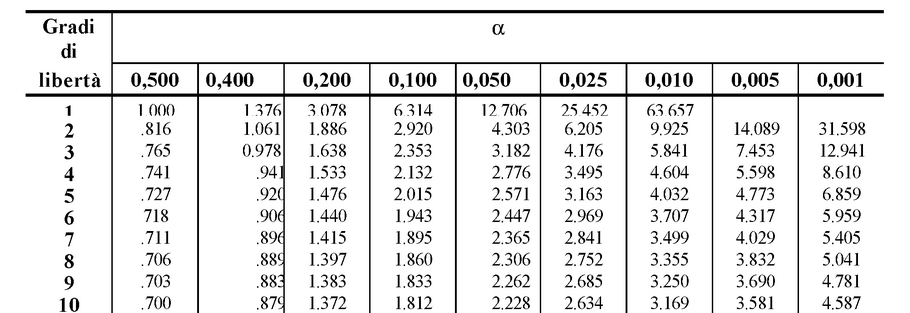
\includegraphics[width=10cm]{tdstudent}};
				\draw (5,1.15) rectangle (5.95,2.75);
				\draw (0.5,1.15) rectangle (5.95,1.45);				
			\end{tikzpicture}
			\caption{Tabella del t di Student a doppia coda}
			\label{fig:}
		\end{figure}
				
		\[t_{5} = 2.571\]
\newpage	
		\subsection{Termocoppia}
		La termocoppia è uno strumento passivo di misura della temperatura: non necessita di alimentazione.
		
		L'input di questo strumento è una temperatura mentre l'output è un $ \Delta V $. Durante l'esercitazione è stato detto che la termocoppia si basa sull’\textit{effetto Seebeck} ovvero sulla migrazione spontanea di elettroni che si manifesta nel momento in cui due conduttori metallici saldati in due giunti distinti vengono sottoposti ad una differenza di temperatura, tale $\Delta T$ genererà un passaggio di elettroni da un giunto ad un altro senza che lo strumento venga alimentato da corrente. 
		
		Al $ \Delta V $ diviene perciò associabile un $\Delta T$, infatti se i giunti sono posti alla stessa temperatura lo strumento misura 0 V. \newline 
		
		Un giunto sarà perciò il riferimento (o giunto freddo) e la sua temperatura andrà conosciuta a priori, nel caso dell'esercitazione questo è stato inserito in una miscela di acqua e ghiaccio a 0 \degree C; l'altro giunto sarà invece quello di misura (o giunto caldo) con cui si mostrerà l'evoluzione temporale della stessa. \newline 
		
		La termocoppia è uno strumento assimilabile ad un primo ordine perché l’elemento sensibile è nient'altro che la punta dove sono saldati i due conduttori, considerabile a massa infinitesima. \newline 
		
		A completare la catena di misura sarà posto un oscilloscopio per la visualizzazione di un segnale in uscita, dove sulle ascisse di questo si vedrà il tempo, mentre sulle ordinate la tensione misurata. 
		
		\begin{figure}[H]
			\centering
			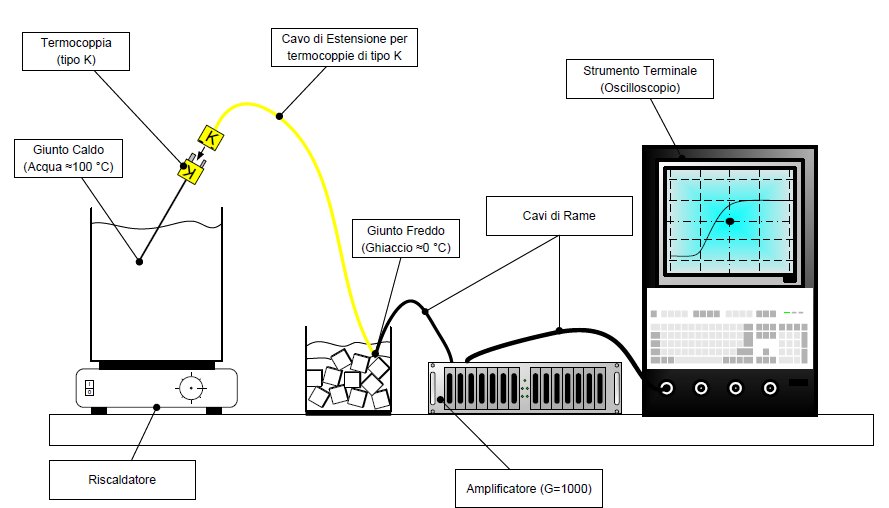
\includegraphics[width=0.5\linewidth]{immagini/catena1}
			\label{fig:catena1}
		\end{figure}		
		
		Tenendo lo strumento tra le dita sull'oscilloscopio si registra un segnale: si è dimostrato lo strumento essere sensibile alla temperatura. 
		
\newpage

		\paragraph{Temperatura Ambiente $\rightarrow$ 100 \degree C} \mbox{}\\
		Allo strumento viene dato un gradino crescente, reagirà quindi con un'esponenziale crescente. \newline
		
		Indicativamente il valore del $\tau$ per esponenziale crescente è posto al 63\% del valore massimo, in questo caso essendo $y_0 = \SI{1900}{\milli\volt}$, il 63\% di $y_0$ vale circa \SI{1200}{\milli\volt} ed incontra il grafico per $\tau=\SI{100}{\milli\second}$.		
		\begin{figure}[H]
			\centering
			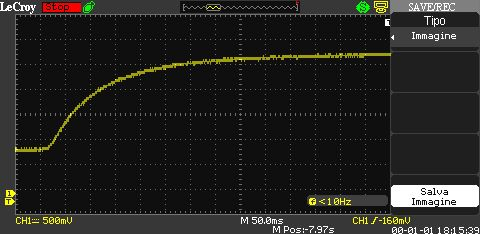
\includegraphics[width=0.7\linewidth]{immaginioscillo/1}
			\caption[]{Transitorio Ambiente - 100 \degree C}
			\label{fig:1}
		\end{figure}	
		Col metodo grafico delle sottotangenti si individuano i seguenti valori di $\tau$, espressi in millisecondi:
		\[ \tau = [57, 79, 100, 102, 83, 133]\]
		Per cui:
		\[\tau_{gr} = \SI[separate-uncertainty = true]{92(27)}{\milli\second}\]		
		\begin{figure}[H]
			\centering
			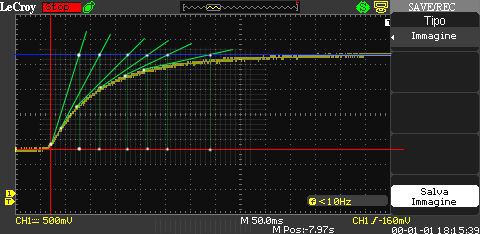
\includegraphics[width=0.7\linewidth]{immaginioscillo/1+}
			\caption{Metodo delle Sottotangenti}
			\label{fig:2}
		\end{figure}	
		Col metodo analitico si scelgono dei valori di tempo $t^*$, dopodiché si individuano i relativi valori di tensione $y(t^*)$, conoscendo $y_0 = \SI{1900}{\milli\volt}$ e applicando la formula inversa trovata per l'esponenziale crescente si otterrà
		\[\tau = - \dfrac{t^*}{\ln\left(y_0-y(t^*)\over y_0\right)}\]		
		\begin{table}[H]
			\centering
			\ra{1.3}
			\begin{tabular}{ccc}
				\toprule
				$t^*$ [\si{\milli\second}] & $y(t^*)$ [\si{\milli\volt}] & $\tau$ [\si{\milli\second}] \\ \midrule
				3                                                     & 100                                                       & 55                                                      \\
				22                                                     & 350                                                       & 108                                                      \\
				55                                                     & 850                                                       & 93                                                      \\
				100                                                     & 1230                                                        & 96                                                      \\
				147                                                     & 1500                                                        & 94                                                      \\
				154                                                     & 1600                                                        & 83                                                      \\ \bottomrule
			\end{tabular}
		\end{table}
		Per cui
		\[\tau_{an} = \SI[separate-uncertainty = true]{88(19)}{\milli\second}\]				
		Il valore di $\tau$ si attesta intorno al valore identificato al 63\% di $y_0$.
\newpage
		\paragraph{100\degree C $\rightarrow$ Temperatura Ambiente}	\mbox{}\\
		Allo strumento viene dato un gradino decrescente, reagirà quindi con un'esponenziale decrescente. \newline
		
		Indicativamente il valore del $\tau$ per esponenziale decrescente è posto al 37\% del valore massimo, in questo caso essendo $y_0 = \SI{2300}{\milli\volt}$, il 37\% di $y_0$ vale circa \SI{850}{\milli\volt} che incontra il grafico per $\tau=\SI{2}{\second}$.		
		\begin{figure}[H]
			\centering
			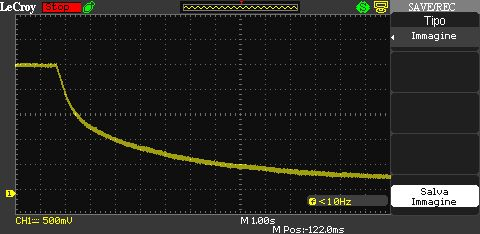
\includegraphics[width=0.7\linewidth]{immaginioscillo/2}
			\caption[]{Transitorio 100 \degree C - Ambiente}
			\label{fig:3}
		\end{figure}		
		Col metodo grafico si individuano i seguenti valori di $\tau$, espressi in secondi:
		\[ \tau = [1, 1.2, 1.8, 2.4, 2.7, 2.7]\]
		Per cui:
		\[\tau_{gr} = \SI[separate-uncertainty = true]{2.0(0.8)}{\second}\]		
		\begin{figure}[H]
			\centering
			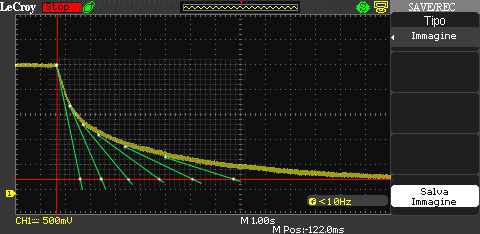
\includegraphics[width=0.7\linewidth]{immaginioscillo/2+}
			\caption{Metodo delle Sottotangenti}
			\label{fig:4}
		\end{figure}		
		Col metodo analitico si scelgono dei valori di tempo $t^*$, dopodiché si individuano i relativi valori di tensione $y(t^*)$, conoscendo $y_0 = \SI{2300}{\milli\volt}$ e applicando la formula inversa trovata per l'esponenziale decrescente si otterrà
		\[\tau = - \dfrac{t^*}{\ln\left(y(t^*)\over y_0\right)} \]		
		\begin{table}[H]
			\centering
			\ra{1.3}
			\begin{tabular}{ccc}
				\toprule
				$t^*$ [\si{\second}] & $y(t^*)$ [\si{\milli\volt}] & $\tau$ [\si{\second}] \\ \midrule
				0.2                                                     & 2000                                                       & 1.4                                                      \\
				0.6                                                     & 1560                                                       & 1.5                                                      \\
				1.1                                                     & 1200                                                       & 1.7                                                      \\
				1.8                                                     & 900                                                        & 1.9                                                      \\
				2.8                                                     & 670                                                        & 2.3                                                      \\
				4.4                                                     & 450                                                        & 2.7                                                      \\ \bottomrule
			\end{tabular}
		\end{table}		
		Per cui
		\[\tau_{an} = \SI[separate-uncertainty = true]{2.0(0.5)}{\second} \]			
		Il valore di $\tau$ si attesta intorno al valore identificato al 37\% di $y_0$. 
\newpage	
		\paragraph{100 \degree C $\rightarrow$ 0 \degree C}	\mbox{}\\
		Allo strumento viene dato un gradino decrescente, reagirà quindi con un'esponenziale decrescente. \newline
		
		Indicativamente il valore del $\tau$ per esponenziale decrescente è posto al 37\% del valore massimo, in questo caso essendo $y_0 = \SI{1650}{\milli\volt}$, il 37\% di $y_0$ vale circa $\SI{610}{\milli\volt}$ che incontra il grafico per $\tau=\SI{150}{\milli\second}$.		
		\begin{figure}[H]
			\centering
			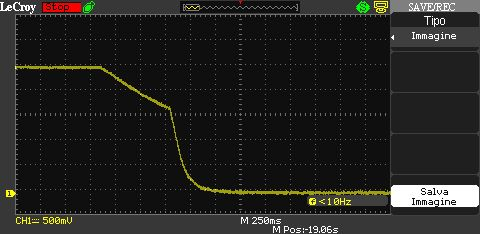
\includegraphics[width=0.7\linewidth]{immaginioscillo/3}
			\caption{Transitorio 100 \degree C - 0 \degree C}
			\label{fig:5}
		\end{figure}		
		Col metodo grafico si individuano i seguenti valori di $\tau$, espressi in millisecondi:
		\[ \tau = [100, 60, 60, 100, 70, 140]\]
		Per cui:
		\[\tau_{gr} = \SI[separate-uncertainty = true]{88(33)}{\milli\second}\]		
		\begin{figure}[H]
			\centering
			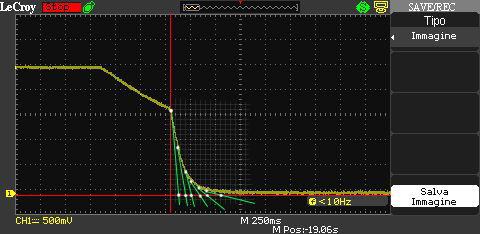
\includegraphics[width=0.7\linewidth]{immaginioscillo/3+}
			\caption{Metodo delle Sottotangenti}
			\label{fig:6}
		\end{figure}		
		Col metodo analitico si scelgono dei valori di tempo $t^*$, dopodiché si individuano i relativi valori di tensione $y(t^*)$, conoscendo $y_0 = \SI{1650}{\milli\volt}$ e applicando la formula inversa trovata per l'esponenziale decrescente si otterrà
		\[\tau = - \dfrac{t^*}{\ln\left(y(t^*)\over y_0\right)} \]		
		\begin{table}[H]
			\centering
			\ra{1.3}
			\begin{tabular}{ccc}
				\toprule
				$t^*$ [\si{\milli\second}] & $y(t^*)$ [\si{\milli\volt}] & $\tau$ [\si{\milli\second}] \\ \midrule
				50                                                     & 1300                                                       & 210                                                      \\
				100                                                   & 930                                                       & 174                                                      \\
				150                                                     & 450                                                       & 115                                                      \\
				300                                                     & 270                                                        & 166                                                      \\
				400                                                     & 130                                                        & 157                                                      \\
				550                                                     & 100                                                        & 196                                                      \\ \bottomrule
			\end{tabular}
		\end{table}		
		Per cui
		\[\tau_{an} = \SI[separate-uncertainty = true]{170(35)}{\milli\second} \]			
		Il valore di $\tau$ individuato col metodo analitico si attesta intorno al valore identificato al 37\% di $y_0$; col metodo grafico si ottiene invece un risultato meno accurato.
							
\newpage	

		\subsection{Quesiti}
		\begin{enumerate}
			\item \textbf{Tabelle Termocoppia} 
			
			\begin{table}[H]
				\centering
				\ra{1.3}
				\captionof{table}{$\tau_{\text{amb}, 100\degree C }$} \label{tab:title} 				
					\begin{tabular}{ccc}
						\toprule
						 \textbf{Misure}                &  \textbf{Metodo Grafico} [ms] &  \textbf{Metodo Analitico} [ms] \\ \midrule
						1                               & 57                   & 55                     \\ 
						2                               & 79                   & 108                    \\ 
						3                               & 100                  & 93                     \\ 
						4                               & 102                  & 96                     \\ 
						5                               & 83                   & 94                     \\ 
						6                               & 133                  & 83                     \\ 
						$\overline{\tau}\pm\varepsilon$ &  $92\pm27$           &  $ 88\pm19 $             \\  \bottomrule
					\end{tabular}			
			\end{table}
			
			\begin{table}[H]
				\centering
				\ra{1.3}
				\captionof{table}{$\tau_{100\degree C, \text{amb}}$} 
				\label{tab:title1} 				
					\begin{tabular}{ccc}
						\toprule
						 \textbf{Misure}                         & \textbf{Metodo Grafic}o [s] &  \textbf{Metodo Analitico} [s] \\ \midrule
						1                               & 1                   & 1.4                   \\ 
						2                               & 1.2                 & 1.5                   \\ 
						3                               & 1.8                 & 1.7                   \\ 
						4                               & 2.4                 & 1.9                   \\ 
						5                               & 2.7                 & 2.3                   \\ 
						6                               & 2.7                 & 2.7                   \\ 
						$\overline{\tau}\pm\varepsilon$ & $ 2.0\pm0.8   $     & $ 2.0\pm0.5  $        \\ \bottomrule
					\end{tabular}
				
			\end{table}
			
			\begin{table}[H]
				\centering
				\ra{1.3}
				\captionof{table}{$\tau_{100\degree C, 0\degree C}$} 
				\label{tab:title3} 
					\begin{tabular}{ccc}
						\toprule
						 \textbf{Misure}                         & \textbf{Metodo Grafico} [ms]  & \textbf{Metodo Analitico} [ms] \\  \midrule
						1                               & 100                  & 210                    \\ 
						2                               & 60                   & 174                    \\ 
						3                               & 60                   & 115                    \\ 
						4                               & 100                  & 166                    \\ 
						5                               & 70                   & 157                    \\ 
						6                               & 140                  & 196                    \\ 
						$\overline{\tau}\pm\varepsilon$ & $ 88\pm33  $         & $ 170\pm35  $          \\ \bottomrule
					\end{tabular}				
			\end{table}

		\item \textbf{Le costanti di tempo calcolate nei diversi transitori sono differenti tra loro? Perché?} \newline
		
		Le costanti di tempo calcolate per i diversi transitori sono diverse perché, di caso in caso, si sta scambiando calore con fluidi dal coefficiente di scambio termico diverso: entrano in gioco condizioni al contorno dettate dalla termo-fluidodinamica. \newline
		
		Nei passaggi da $ T_{amb} \rightarrow $ 100 \degree C e da 100 \degree C $\rightarrow$ 0 \degree C sia la curva che la misura sono più rapide perché si torna a scambiare calore in acqua, fluido caratterizzato da un coefficiente convettivo pari a		
		\[h_{acqua} = 500\div10~000~\unit{\watt\per\square\meter\per\kelvin}\]		
		Al contrario, il transitorio da 100 \degree C $\rightarrow T_{amb}$ è più lento dato che si sta scambiando calore in aria, fluido caratterizzato da un coefficiente convettivo pari a 		
		\[h_{aria} = 10\div100~\unit{\watt\per\square\meter\per\kelvin}  \]		
		Il coefficiente convettivo di scambio termico dell’aria è più basso di quello dell’acqua di almeno due ordini di grandezza determinando così un transitorio dello strumento più lento ed una costante di tempo dal valore più alto.
		
\newpage		

		\item \textbf{Con riferimento al transitorio relativo al passaggio tra 100\degree C a 0\degree C, si calcoli il tempo di stabilizzazione nell’ipotesi di un errore dinamico di $ \varepsilon_d = \pm5\% $.} \newline 
		
		Il Tempo di stabilizzazione $ T_{st} $ è il tempo necessario affinché il segnale entri all’interno della banda di errore dinamico $ \varepsilon_d $ e non esca più.
		
		È richiesta una banda di errore dinamico del $ \pm5\% $ di $ y_0 $, per cui sarà circa compresa tra i valori di $\pm80\,\text{mV}$. 
		\begin{figure}[H]
			\centering
			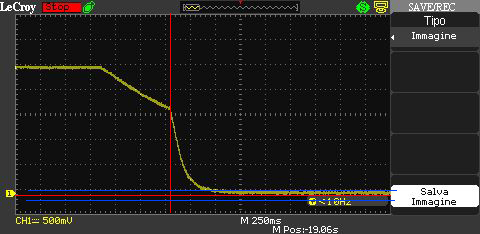
\includegraphics[width=0.7\linewidth]{immaginioscillo/3+banda}
			\caption{Banda di errore dinamico in blu}
			\label{fig:3banda}
		\end{figure}
		Il tempo che impiega il segnale ad entrare nella banda di errore dinamico per non uscire più è pari a:
		\[T_{st} = \SI{500}{\milli\second}\]
		
		\item \textbf{Con riferimento al transitorio relativo al passaggio tra temperatura ambiente e 100 \degree C, si calcoli la banda passante del sistema.} \newline
		
		La banda passante dello strumento è quell'intervallo caratterizzato da tutte quelle frequenze tali per cui la deamplificazione del segnale sia minore di $\SI{3}{\dB}$. Questa nel caso in esame sarà pari a:
		\[[0; f_t]\]
		Con $f_t$ frequenza di taglio alla quale si ha deamplificazione del guadagno pari a $ \SI{3}{\dB}$.
		\[\omega_t = 2\pi f_t = {1\over\tau} \Rightarrow f_t = \dfrac{1}{2\pi\tau}\]
		Attraverso il metodo grafico il tempo caratteristico del transitorio da temperatura ambiente a 100\degree C era
		\[\tau_{gr} = \SI[separate-uncertainty = true]{92(27)}{\milli\second}\]		
		Il valore della frequenza di taglio è pari a:
		\[ f_t\footnote{Si è scelta di mantenere questa unità di misura, consci che [\si{\hertz}]=[\si{\per\second}] 
			per personali motivi di semplicità di visualizzazione, e in più non compare alcuna pulsazione 
			con la quale possa confondersi.} = \dfrac{1}{2\pi\tau} = \dfrac{1}{2\pi\cdot \SI{92}{\milli\second}} = \SI{1.7d-3}{\per\milli\second}\]
		Per il calcolo dell'incertezza legata a questa misura ci si affida alla valutazione effettuata per grandezze indipendenti. 
		
		L'incertezza legata alla $\tau$ è l'incertezza estesa $U = \SI{27}{\milli\second} $, attraverso il valore del $t$ di Student utilizzato si trova che la sua incertezza standard è pari a:
		\[ u_\tau = \dfrac{U}{t_{gdl}} = {\SI{27}{\milli\second}\over2.571} = \SI{10.5}{\milli\second}\]
		\[{\partial f_t\over\partial\tau} = -\dfrac{1}{2\pi\tau^2} = \SI{-1,88d-5}{\per\square\milli\second}\]
		\[ \begin{aligned}
			u_{f_t} & = \sqrt{\left({\partial f_t\over\partial\tau}\right)^2\cdot u_\tau^2 } = \sqrt{ \Biggl[\SI{-1,88d-5}{\per\square\milli\second}\Biggr]^2 \cdot \Biggl[\SI{10.5}{\milli\second}\Biggr]^2} = \\
			& = \sqrt{\SI{3.8967d-8}{\per\square\milli\second}} = \SI{1.97d-4}{\per\milli\second}
		\end{aligned}\]
		Che moltiplicato per il coefficiente di copertura $k$ dato dalla distribuzione $t$ di Student per una fiducia del 95\% $ k=2.571 $, porta ad un'incertezza estesa pari a:
		\[ U_{f_t} = k\cdot u_{f_t} = \SI{5.0d-4}{\per\milli\second}\]
		Infine, il valore della frequenza di taglio sarà:
		\[f_t = \SI[separate-uncertainty = true]{1.7(0.5)d-3}{\per\milli\second}\]
		E la banda passante sarà data da:
		\[ [0; f_t]\]
		\end{enumerate}

\newpage

		\subsection{Termistore}
		Dopo la termocoppia, il secondo strumento del primo ordine provato è stato il termistore. Anche questo misura una temperatura e durante l'esercitazione è stato detto che, a differenza della termocoppia, è uno strumento a variazione di resistenza. 
		
		La resistenza è proporzionale alla lunghezza e allo spessore del materiale attraverso la resistività, essendo quest'ultima variabile con la temperatura diviene così possibile misurare una variazione di resistenza attraverso una variazione di temperatura. 
		
		Poiché una variazione di resistenza per essere misurata ha bisogno di una corrente, il termistore è uno strumento attivo. 
		
		Il termistore viene solitamente collegato postumo ad un partitore di tensione, questo perché ai fini misuristici si vuole misurare un $ \Delta V $ piuttosto che un $ \Delta R $.
		
		Il termistore dell’esperienza non ha un partitore incorporato per cui se ne è aggiunto uno per facilitare la misurazione del delta $ \Delta R $. \newline		
		
		Il termistore analizzato è di tipo NTC, l’andamento del parametro è inverso rispetto a ciò che è stato visto in teoria: al gradino crescente risponderà con un gradino decrescente, perciò all'aumentare della temperatura diminuirà la resistenza, e viceversa. 
		
		L’\textit{"N"} in acronimo è inoltre indice che questi termistori vengono realizzati con dei semiconduttori a drogaggio N. \newline
		
		Anche in questo caso essendo l'elemento sensibile una propaggine conduttiva praticamente priva di inerzia e quindi a massa trascurabile, il termistore ricade nel gruppo degli strumenti del primo ordine. 
		
\newpage
		
		\paragraph{Termistore a pelo libero: 0 \degree C$\rightarrow$100 \degree C} \mbox{}\\
		Si proceda con l'acquisizione di un singolo gradino crescente. \newline 
		
		Indicativamente il valore del $\tau$ per esponenziale decrescente è posto al 37\% del valore massimo, in questo caso essendo $y_0 = \SI{1200}{\milli\volt}$, il 37\% di $y_0$ vale circa $\SI{440}{\milli\volt}$ che incontra il grafico per $\tau=\SI{600}{\milli\second}$.		
		\begin{figure}[H]
			\centering
			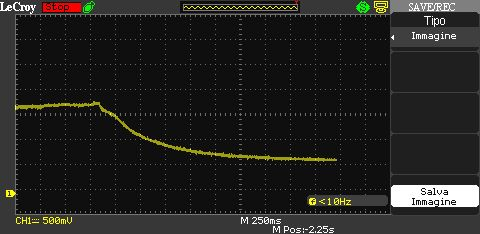
\includegraphics[width=0.7\linewidth]{immaginioscillo/4}
			\caption{Transitorio 0 \degree C $\rightarrow$ 100 \degree C}
			\label{fig:7}
		\end{figure}				
		Col metodo grafico si individuano i seguenti valori di $\tau$, espressi in millisecondi:
		\[ \tau = [250,\, 600,\, 575,\, 600,\, 500,\, 550]\]
		Per cui:
		\[\tau_{gr} = \SI[separate-uncertainty = true]{512(141)}{\milli\second}\]		
		\begin{figure}[H]
			\centering
			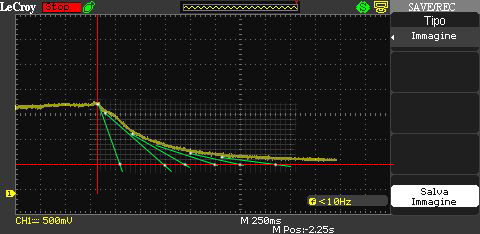
\includegraphics[width=0.7\linewidth]{immaginioscillo/4+}
			\caption{Metodo delle Sottotangenti}
			\label{fig:8}
		\end{figure}		
		Il valore ottenuto col metodo grafico si attesta intorno al valore identificato al 37\% di $y_0$.	

		\paragraph{Termistore incapsulato: 0\degree C$\rightarrow$100\degree C} \mbox{}\\
		Si proceda con l'acquisizione di un singolo gradino crescente. \newline 
		
		Indicativamente il valore del $\tau$ per esponenziale decrescente è posto al 37\% del valore massimo, in questo caso essendo $y_0 = \SI{2000}{\milli\volt}$, il 37\% di $y_0$ vale circa $\SI{740}{\milli\volt}$ che incontra il grafico per $\tau=\SI{5.5}{\second}$.		
		\begin{figure}[H]
			\centering
			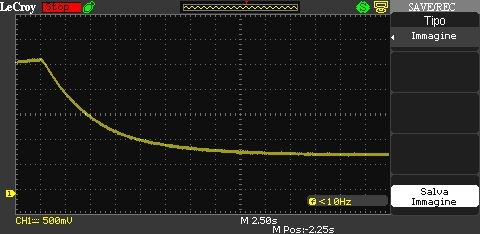
\includegraphics[width=0.7\linewidth]{immaginioscillo/5}
			\caption{Transitorio 0 \degree C $\rightarrow$ 100 \degree C}
			\label{fig:9}
		\end{figure}				
		Col metodo grafico si individuano i seguenti valori di $\tau$, espressi in secondi:
		\[ \tau = [4.75,\, 5.85,\, 6,\, 6,\, 6.5,\, 7]\]
		Per cui:
		\[\tau_{gr} = \SI[separate-uncertainty = true]{6(1)}{\second}\]				
		\begin{figure}[H]
			\centering
			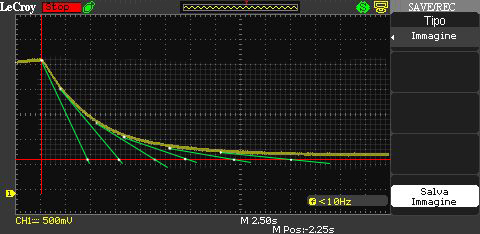
\includegraphics[width=0.7\linewidth]{immaginioscillo/5+}
			\caption{Metodo delle Sottotangenti}
			\label{fig:10}
		\end{figure}		
		Il valore ottenuto col metodo grafico si attesta intorno al valore identificato al 37\% di $y_0$.	
		
\newpage	
		
		\subsection{Quesiti}
		\begin{enumerate}
			\item \textbf{Tabelle Termistore}	
					
				\begin{table}[H]
					\centering
					\ra{1.3}
					\captionof{table}{$\tau_{0\degree C, 100\degree C}$ a pelo libero} 
					\label{tab:title4} 				
				\begin{tabular}{cc}
					\toprule
					\textbf{Misure}                 & \textbf{Metodo Grafico} [ms] \\ \midrule
					1                               & 250                  \\ 
					2                               & 600                  \\ 
					3                               & 575                  \\ 
					4                               & 600                  \\ 
					5                               & 500                  \\ 
					6                               & 550                  \\ 
					$\overline{\tau}\pm\varepsilon$ & $ 512\pm141 $        \\ \bottomrule 
				\end{tabular}			
			\end{table}
		
			\begin{table}[H]
				\centering
				\ra{1.3}
				\captionof{table}{$\tau_{0\degree C, 100\degree C}$ con involucro} 
				\label{tab:title5} 
		\begin{center}
			\begin{tabular}{cc}
				\toprule
				\textbf{Misure}                 & \textbf{Metodo grafico} [s] \\ \midrule
				1                               & 4,75                \\ 
				2                               & 5,85                \\ 
				3                               & 6                   \\ 
				4                               & 6                   \\ 
				5                               & 6,5                 \\ 
				6                               & 7                   \\ 
				$\overline{\tau}\pm\varepsilon$ & $ 6\pm1 $           \\	\bottomrule 
			\end{tabular}
		\end{center}
		\end{table}
	
\newpage	

		\item \textbf{Riportare le motivazioni per cui i due termistori hanno costanti di tempo diverse tra loro. \\ Giustificare le risposte.} 
		
		\[\tau_{gr}^{\text{libero}} = \SI[separate-uncertainty = true]{512(141)}{\milli\second}\]		
		\[\tau_{gr}^{\text{involucro}} = \SI[separate-uncertainty = true]{6(1)}{\second}\]				
		La motivazione per cui le due costanti di tempo sono diverse risiede nella termodinamica. 
		
		L'elemento sensibile dello strumento nella prima applicazione è libero, mentre nella seconda è racchiuso da un involucro protettivo. Questo involucro, seppur considerandolo a massa trascurabile, rende lo strumento meno rapido a causa dell'inevitabile aumento di massa: prima che la misura avvenga sull'elemento sensibile al suo interno, dovrà necessariamente scaldarsi prima l'involucro.
		\end{enumerate}
	
\newpage	
	
		\section{Parte 2: Sistemi del secondo ordine} 
		\subsection{Misura sperimentale dei parametri dinamici}
		Un sistema del secondo ordine è caratterizzato da una risposta in frequenza definita da due parametri: la pulsazione propria $\omega_0$ e lo smorzamento $\xi$. \newline
		
		In questa esperienza si calcoleranno graficamente i parametri dinamici attraverso il calcolo del decremento logaritmico $\delta$.
		\[\delta = {1\over n}\ln\left(y_n\over y_{n+m}\right) = \dfrac{2\pi\xi}{\sqrt{1-\xi^2}}\]
		Con $n$ ordine del massimo scelto ed $y$ ampiezza dell'oscillazione dal valore asintotico. \newline 
		
		Calcolando il decremento logaritmico attraverso l'immagine ottenuta dall'oscilloscopio si può ricavare lo smorzamento: 
		\[\delta = \dfrac{2\pi\xi}{\sqrt{1-\xi^2}} \Rightarrow \xi = \dfrac{\delta}{\sqrt{4\pi^2 + \delta^2}}\]  
		
		In più individuando lo pseudoperiodo $T_0$ tra i massimi di ordine $n$ ed $n+m$ scelti, si possono calcolare:
		\begin{itemize}
		\item La pulsazione propria:
		\[\omega_0 = {2\pi\over T_0}\] 
		\item La pulsazione naturale:
		\[\omega_n = \dfrac{2\pi}{T_0\sqrt{1-\xi^2}}\]
		\item La frequenza naturale:
		\[f_n = {\omega_n\over2\pi}\]
		\end{itemize}
		L’andamento nel tempo di un sistema del secondo ordine sottosmorzato $\xi<1$ è una sinusoide smorzata, mentre un sistema sovrasmorzato $\xi>1$ reagisce grossomodo come un sistema del primo ordine.
		\[y(t) = Ae^{-\omega_n\xi t}\sin(\omega_0t+\varphi)\]
		
\newpage
		
		\subsection{Cella di carico}
		
		La massa ora non è più trascurabile.\newline
		
		La cella di carico è uno strumento attivo che misura forze. Nel caso in esame questa è composta da una trave incastrata e da due coppie di estensimetri, questi saranno in grado di leggere le deformazioni e trasformarle in una grandezza visualizzabile mediante un oscilloscopio. 
		
		Gli elementi sensibili della cella di carico sono gli estensimetri i quali, attraverso delle resistenze, misureranno una deformazione. 
		
		In output dall'estensimetro si registrerà un $\Delta R$, questo è legato  - attraverso la resistività - alle caratteristiche geometriche del materiale, per cui variando lunghezza e spessore dello stesso varierà la resistenza. 		
		
		Il $\Delta R$ in output per divenire facilmente leggibile viene convertito in un $\Delta V$ mediante la configurazione degli estensimetri a \textit{Ponte di Wheatstone}: questo permetterà di tradurre una forza che provocherà una deformazione (letta dagli estensimetri come un $\Delta R$) in un $\Delta V$ osservabile attraverso uno strumento terminale. 
		
		A completare la catena di misura, oltre al blocco di alimentazione e all'amplificatore, si avrà un oscilloscopio che permetterà la visualizzazione del segnale. 
		
		\begin{figure}[H]
			\centering
			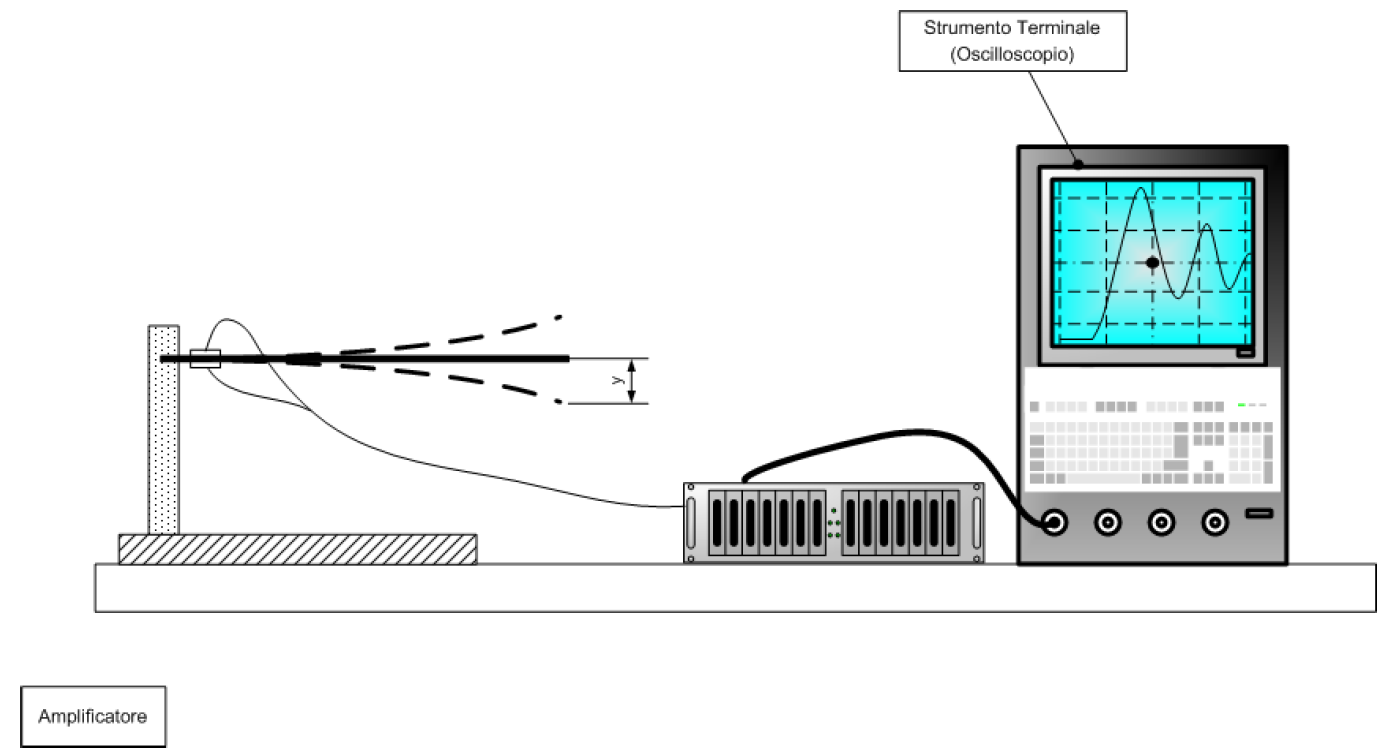
\includegraphics[width=0.7\linewidth]{immagini/catena2}
			\label{fig:catena2}
		\end{figure}
		
		 Mentre in un termometro a resistenza è la deformazione data dai gradienti termici ad essere una grandezza di influenza; nella misurazione della deformazione attraverso estensimetri a resistenza è la temperatura, rea di indurre deformazioni, ad essere una grandezza di influenza.
\newpage		 
		 \subsection{Evoluzioni Libere}
		 Le prime che si acquisiscono sono tre evoluzioni libere senza massa. La prima testa il funzionamento della cella di carico e aggiunta alla successive permette di stabilire, attraverso il calcolo grafico del decremento logaritmico, i valori dei parametri caratteristici degli strumenti del secondo ordine. 
		 
		 \paragraph{Prima evoluzione libera} \mbox{} \\
		 \begin{figure}[H]
		 	\centering
		 	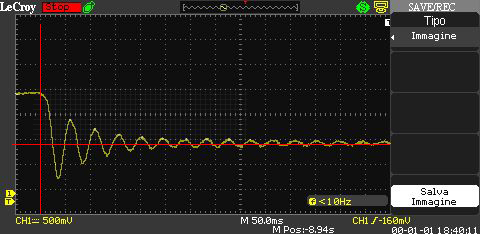
\includegraphics[width=0.6\linewidth]{immaginioscillo/6+}
		 	\caption{Prima evoluzione libera}
		 	\label{fig:11}
		 \end{figure}
	 
	 	Il massimo di ordine $ 0 $ che si sceglie ha ordinata pari a $y_{\max}=\SI{500}{\milli\volt}$, si scelgono poi i massimi di ordine $n=1$ ed $n=2$ rispettivamente caratterizzati dai seguenti valori di pseudoperiodo ed ordinate:
	 	\[T^1_0=\SI{50}{\milli\second};\quad  T_0^2=\SI{100}{\milli\second}\]
	 	\[y^1_{\max}=\SI{300}{\milli\volt};\quad  y_{\max}^2=\SI{300}{\milli\volt}\]
	 	
\newpage	 	
	 	
	 	\paragraph{Seconda evoluzione libera} \mbox{} \\
	 	\begin{figure}[H]
	 		\centering
	 		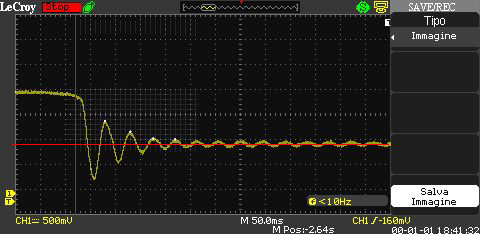
\includegraphics[width=0.6\linewidth]{immaginioscillo/7+}
	 		\caption{Seconda evoluzione libera}
	 		\label{fig:12}
	 	\end{figure}
	 	Il massimo di ordine 0 che si sceglie ha ordinata pari a $y_{\max}=\SI{450}{\milli\volt}$, si scelgono poi i massimi di ordine $n=1$ ed $n=2$ rispettivamente caratterizzati dai seguenti valori di pseudoperiodo ed ordinate: 
	 	\[T^1_0=\SI{50}{\milli\second};\quad  T_0^2=\SI{95}{\milli\second}\]
	 	\[y^1_{\max}=\SI{250}{\milli\volt};\quad  y_{\max}^2=\SI{100}{\milli\volt}\]
	 
	 	
	 	\paragraph{Terza evoluzione libera} \mbox{} \\
	 	\begin{figure}[H]
	 		\centering
	 		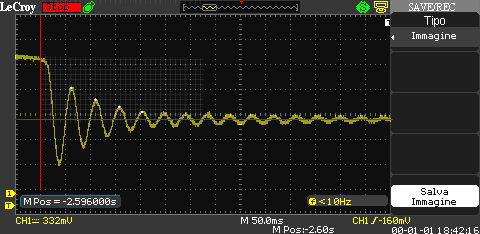
\includegraphics[width=0.6\linewidth]{immaginioscillo/8+}
	 		\caption{Terza evoluzione libera}
	 		\label{fig:13}
	 	\end{figure}
	 	Il massimo di ordine 0 che si sceglie ha ordinata pari a $y_{\max}=\SI{398}{\milli\volt}$, si scelgono poi i massimi di ordine $n=1$ ed $n=2$ rispettivamente caratterizzati dai seguenti valori di pseudoperiodo ed ordinate:
	 	\[T^1_0=\SI{50}{\milli\second};\quad  T_0^2=\SI{97}{\milli\second}\]
	 	\[y^1_{\max}=\SI{266}{\milli\volt};\quad  y_{\max}^2=\SI{134}{\milli\volt}\]

\newpage
	 	
	 	\subsection{Evoluzioni con massa}
	 	Alla lamina ora si aggiungono due masse note supplementari. \newline
	 	
	 	In uscita ci si aspetta un'oscillazione minore: ricordando che $\omega=\sqrt{k\over m}$ aumentando la massa diminuirà la pulsazione e al secondo si registreranno meno oscillazioni e occorrerà più tempo per arrivare all'asintoto.
	 	
	 	\paragraph{Evoluzione con $1\,\text{kg}$} \mbox{} \\ 
	 	\begin{figure}[H]
	 		\centering
	 		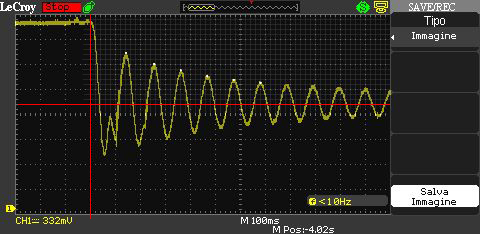
\includegraphics[width=0.7\linewidth]{immaginioscillo/9+}
	 		\caption{Evoluzione con $1\,\text{kg}$}
	 		\label{fig:14}
	 	\end{figure}
 	
	 	Il massimo di ordine 0 che si sceglie ha ordinata pari a $y_{\max}=\SI{664}{\milli\volt}$, si sceglie poi il massimo di ordine $n=1$ caratterizzato dai seguenti valori di pseudoperiodo ed ordinate:
	 	\[T_0=\SI{130}{\milli\second};\quad  y^1_{\max}=\SI{531}{\milli\volt}\]

\newpage
	 	
	 	\paragraph{Evoluzione con $2\,\text{kg}$} \mbox{} \\ 
	 	\begin{figure}[H]
	 		\centering
	 		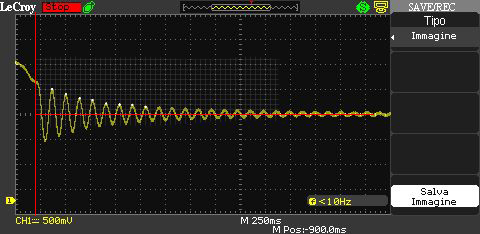
\includegraphics[width=0.7\linewidth]{immaginioscillo/10+}
	 		\caption{Evoluzione con $2\,\text{kg}$}
	 		\label{fig:15}
	 	\end{figure}
	 	Il massimo di ordine 0 che si sceglie ha ordinata pari a $y_{\max}=\SI{500}{\milli\volt}$, si sceglie poi il massimo di ordine $n=3$ caratterizzato dai seguenti valori di pseudoperiodo ed ordinate: 
	 	\[T_0=\SI{950}{\milli\second};\quad  y^1_{\max}=\SI{300}{\milli\volt}\]
	 	
\newpage	 	

	 	\subsection{Quesiti}
	 	\begin{enumerate}
	 		\item \textbf{Compilare la tabella sottostante utilizzando i grafici acquisiti nelle evoluzioni libere in presenza di massa. Attenzione a riportare per ogni grandezza la corretta unità di misura.}
	 		
	 		\begin{table}[H]
	 			\centering
	 			\ra{1.3}
	 			\captionof{table}{Evoluzioni con massa} 
	 			\label{tab:title6} 
	 			\begin{tabular}{ccccccc}
	 				\toprule
	 				\textbf{Evoluzioni}  &  $\delta$ &  $ T_0~[\text{ms}] $ &  $\omega_0~[\text{ms}^{-1}]$&  $\xi$ &  $\omega_n~[\text{ms}^{-1}]$&  $f_n~[\text{mHz}]$ \\ \midrule
	 				1 kg        & 0.223     & 130                  & 0.048                       & 0.035  & 0.048                       & 0.008              \\ 
	 				2 kg        & 0.170     & 950                  & 0.007                       & 0.027  & 0.007                       & 0.001              \\ \bottomrule
	 			\end{tabular}
	 		\end{table}
% 		Scrivendo per esteso le pulsazioni naturali e quelle proprie dei due sistemi, \textsc{Matlab} fornisce: 
% 		\[\omega_0^{1\,\text{kg}} = 0,0483321946706122\,\text{ms}^{-1}  \qquad \omega_n^{1\,\text{kg}} = 0,0483933606670632\,\text{ms}^{-1}\]
% 		Con un errore relativo di:\(\qquad6\cdot10^{-5}\,\text{ms}^{-1}\)
% 		\[\omega_0^{2\,\text{kg}} = 0,00661387927071535\,\text{ms}^{-1}  \qquad \omega_n ^{2\,\text{kg}} = 0,00661873662034488\,\text{ms}^{-1}\]
% 		Con un errore relativo di:\(\qquad5\cdot10^{-6}\,\text{ms}^{-1}\) \newline
% 		
% 		Sebbene per via grafica si era intuito, calcolando le frequenze proprie e di risonanza dei sistemi, queste differiscono tra loro in un caso per $10^{-5}$ e nell'altro per $10^{-6}$, si può assumere quindi che, per entrambi i sistemi:
% 		\[\omega_n = \omega_0\]
% 		Concludendo che sono in risonanza. 
 		
 		\item \textbf{Compilare la tabella sottostante calcolando almeno due decrementi logaritmici per ogni grafico acquisito nelle due (tre) evoluzioni libere in assenza di massa. Attenzione a riportare per ogni grandezza la corretta unità di misura. Per il calcolo dell’incertezza si trascurino le componenti legate alla strumentazione presente nella catena di misura.}
 		
 		\begin{table}[H]			
 			\ra{1.3}
 			\captionof{table}{Evoluzioni libere} 
 			\label{tab:title7}
 			\hspace{-1.5cm}  				
 				\begin{tabular}{cccccccc}
 					\toprule
 					\textbf{Evoluzioni}   &  \textbf{Misure}               &  $\delta$ &  $T_0~[\text{ms}] $  & $\omega_0~[\text{ms}^{-1}]$  & $\xi$           & $\omega_n~[\text{ms}^{-1}]$  & $f_n~[\text{mHz}]$ \\ \midrule
 					\multirow{2}*{1}      & 1                              & 0.51      & 50                   & 0.12                         & 0.08            & 0.17                         & 0.027              \\ 
 					                      & 2                              & 0.46      & 100                  & 0.06                         & 0.07            & 0.08                         & 0.013              \\ \hline
 					\multirow{2}*{2}      & 1                              & 0.59      & 50                   & 0.12                         & 0.09            & 0.19                         & 0.030              \\ 
 					                      & 2                              & 0.75      & 95                   & 0.07                         & 0.12            & 0.15                         & 0.024              \\ \hline
 					\multirow{2}*{3}      & 1                              & 0.40      & 50                   & 0.12                         & 0.06            & 0.15                         & 0.024              \\ 
 					                      & 2                              & 0.55      & 97                   & 0.06                         & 0.09            & 0.09                         & 0.015              \\ \hline
 					                      & $\overline{\mu}\pm\varepsilon$ & ~         & ~                    & ~                            & $ 0.09\pm0.05 $ & $ 0.14\pm0.05 $              & $ 0.022\pm0.007 $  \\ \bottomrule
 				\end{tabular}		
 		\end{table}
 		
 		Il calcolo dell'errore si esegue sempre passando attraverso i valori di confidenza ed il t di student. 
 		
 		Per una confidenza del $95\%$ ed un numero di 6 campioni, si individua 
 		\[t_5 = 2.571\]
 
\newpage
 	
 		\item \textbf{Considerando le misure effettuate con masse 1.0 kg e 2.0 kg, riportare l’equazione del rapporto delle due pulsazioni naturali in funzione delle due masse. Calcolare l’errore relativo considerando quanto ricavato sperimentalmente.}
 		\[\frac{\omega_n^{2\,\text{kg}}}{\omega_n^{1\,\text{kg}}} = \dfrac{\sqrt{\frac{k_{\text{trave}}}{M_2}}}{\sqrt{\frac{k_{\text{trave}}}{M_1}}} = \sqrt{\dfrac{\frac{\cancel{k_{\text{trave}}}}{M_2}}{\frac{\cancel{k_{\text{trave}}}}{M_1}}} = \sqrt{\dfrac{M_1}{M_2}}\]
 		\[\frac{\omega_n^{2\,\text{kg}}}{\omega_n^{1\,\text{kg}}} = \dfrac{\SI{0.007}{\per\milli\second}}{\SI{0.048}{\per\milli\second}} = 0.146 \hspace{3cm} \sqrt{\dfrac{M_1}{M_2}} = 0.707\]
 		
 		Con un errore relativo di:~\num{5.6d-1} \newline 
 		
 		Ovvero due rapporti differiscono del: 
 		\[\Delta\%=\left|\dfrac{0,146-0,707}{0,707}\right|\cdot100 = 79.35\]
 		\[79\%\]
	 	\end{enumerate}
		 
\newpage
\newgeometry{top=0.5cm, bottom=0.5cm, left=0.5cm, right=0.5cm}	
\section{Codici Matlab}		
\subsection{Sistemi del primo ordine}
\footnotesize 
\begin{verbatim}
	% Strumento del primo ordine 
	% CONTROLLA CHE TIPO DI ESPONENZIALE HAI
	% ALLE RIGHE 55-49
	
	close all
	clear all
	clc
	format loose
	format short
	
	%% METODO GRAFICO
	V = input('Inserisci tra [] i valori che hai trovato:');
	
	% La media di tali valori è
	tau_gr = mean(V);
	
	fprintf('La media di tali valori è: %3.1f \n', tau_gr);
	
	% La somma degli scarti al quadrato è:
	z_gr = sum((V-tau_gr).^2);
	
	% La deviazione standard è: 
	d_gr = sqrt(z_gr/(length(V)-1));
	fprintf('La deviazione standard  di tali valori è: %3.1f \n', d_gr);
	
	% Solitamente alpha = 0.05, t sceglilo dalla tabella in funzione dei tuoi
	% gradi di libertà:
	t_gr = input('Cerca in tabella e inserisci il t del livello di signficatività che vuoi:'); 
	
	% L'incertezza è:
	e_gr = t_gr*(d_gr/sqrt(length(V)));
	fprintf('L''incertezza associata a tali valori è: \xB1 %3.1f \n', e_gr);
	
	% Riultato finale col metodo grafico è...
	fprintf('Il riultato finale col metodo grafico è: %3.1f \xB1 %3.1f \n', tau_gr, e_gr);

	%% METODO ANALITICO
	% Valore iniziale/massimo: 
	y_0 = input('Fornisci il valore di y_{0}:');
	
	% Coppia di valori letti sul grafico:
	t_sg  = input('Fornisci tra [] i valori di t^{*}:');
	y_sg = input('Fornisci tra [] i valori di y^{*}:');
	
	% Valori delle costanti di tempo calcolate dalle coppie di valori
	% considerate:
	
	% Esponenziale crescente 
	% tau_i = -t_sg./(log((y_0-y_sg)./y_0));
	
	% Esponenziale decrescente
	tau_i = -t_sg./(log(y_sg./y_0));
	
	disp(tau_i')
	
	% Calcolo della media:
	tau = mean(tau_i);
	fprintf('La media di tali valori è: %3.1f \n', tau);
	
	% Somma degli scarti al quadrato:
	z_an = sum((tau_i-tau).^2);
	
	% Deviazione standard:
	d_an = sqrt(z_an/(length(tau_i)-1));
	fprintf('La deviazione standard di tali valori è: %3.1f \n', d_an);
	
	% Significatività:
	t_an = input('Cerca in tabella e inserisci il t del livello di signficatività che vuoi:');
	
	% Incertezza:
	e_an = t_an*(d_an/sqrt(length(tau_i)));
	fprintf('L''incertezza associata a tali valori è: \xB1 %3.1f \n', e_an);
	
	% Riultato finale col metodo analitico è...
	fprintf('Il riultato finale col metodo analitico è: %3.1f \xB1 %3.1f \n', tau, e_an);
	
	%% Tabulazione termocoppia
	V(7) = tau_gr;
	V(8) = e_gr;
	tau_i(7) = tau;
	tau_i(8) = e_an;
	
	M = 'Media'; I = 'Incertezza'; 
	Prove = [1; 2; 3; 4; 5; 6; 7; 8]; Procedimento1 = V'; Procedimento2 = tau_i';
	% t = table(Prove, Procedimento1, Procedimento2) 
	% writetable(t,'Termocoppia 100 - 0.xlsx');
	
	
	%% Tabulazione termistore 
	V(7) = tau_gr;
	V(8) = e_gr;
	Prove = [1; 2; 3; 4; 5; 6; 7; 8]; Procedimento1 = V';
	% t = table(Prove, Procedimento1) 
	% writetable(t,'Termistore 0-100 involucro.xlsx');	
\end{verbatim}
			
\subsection{Strumenti del secondo ordine}
\subsubsection{Evoluzioni libere}
 \footnotesize
\begin{verbatim}
	%Strumento del secondo ordine - evoluzioni libere
		
	close all
	clear all
	clc
	
	%% PRIMA EVOLUZIONE LIBERA
	% Metodo grafico, calcolo del decremento logaritmoco
	
	% Ordine dei massimi, per un massimo dopo l'altro N = 1
	prompt = input('PRIMA EVOLUZIONE LIBERA, premi INVIO per procedere...', "s"); %Stringa
	N1 = input('Quale ordine di massimi scegli? [N1, N2]:');
	y_max1= input('Y_{max, 0}: Valore del massimo di ordine 0:');
	y_maxi1 = input('Y_{max,N}: Valori dei massimi di ordine N individuati [Y_{max,1}, Y_{max,2}]:'); 
	d1 = (1./N1).*log(y_max1./y_maxi1);
	
	fprintf('Il decremento logaritmico è pari a %f \n', d1);
	
	% Smorzamento
	z1 = d1./sqrt(4*pi^2 + d1.^2);
	
	fprintf('I coefficienti di smorzamento sono: %f \n', z1);
	
	% Periodo
	T_01 = input('Inserisci i valori dei periodi tra i massimi che hai considerato [T1,T2]:');
	
	% Pulsazione propria 
	w_01 = (2*pi)./T_01;
	
	% Pulsazione naturale
	w_n1 = (2*pi)./(T_01.*(1-d1.^2));
	
	% Frequenza naturale 
	f_n1 = w_n1./(2*pi);
	
	%% SECONDA EVOLUZIONE LIBERA
	% Metodo grafico, calcolo del decremento logaritmoco
	
	% Ordine dei massimi, per un massimo dopo l'altro N = 1
	prompt = input('SECONDA EVOLUZIONE LIBERA, premi INVIO per procedere...', "s");
	N2 = input('Quale ordine di massimi scegli? [N1, N2]:');
	y_max2= input('Y_{max, 0}: Valore del massimo di ordine 0:');
	y_maxi2 = input('Y_{max,N}: Valori dei massimi di ordine N individuati [Y_{max,1}, Y_{max,2}]:'); 
	d2 = (1./N2).*log(y_max2./y_maxi2);
	
	fprintf('Il decremento logaritmico è pari a %f \n', d2);
	
	% Smorzamento
	z2 = d2./sqrt(4*pi^2 + d2.^2);
	
	fprintf('I coefficienti di smorzamento sono: %f \n', z2);
	
	% Periodo
	T_02 = input('Inserisci i valori dei periodi tra i massimi che hai considerato [T1,T2]:');
	
	% Pulsazione propria 
	w_02 = (2*pi)./T_02;
	
	% Pulsazione naturale
	w_n2 = (2*pi)./(T_02.*(1-d2.^2));
	
	% Frequenza naturale 
	f_n2 = w_n2./(2*pi);
	
	
	%% TERZA EVOLUZIONE LIBERA
	% Metodo grafico, calcolo del decremento logaritmoco
	
	% Ordine dei massimi, per un massimo dopo l'altro N = 1
	prompt = input('TERZA EVOLUZIONE LIBERA, premi INVIO per procedere...', "s");
	N3 = input('Quale ordine di massimi scegli? [N1, N2]:');
	y_max3= input('Y_{max, 0}: Valore del massimo di ordine 0:');
	y_maxi3 = input('Y_{max,N}: Valori dei massimi di ordine N individuati [Y_{max,1}, Y_{max,2}]:'); 
	d3 = (1./N3).*log(y_max3./y_maxi3);
	
	fprintf('Il decremento logaritmico è pari a %f \n', d3);
	
	% Smorzamento
	z3 = d3./sqrt(4*pi^2 + d3.^2);
	
	fprintf('I coefficienti di smorzamento sono: %f \n', z3);
	
	% Periodo
	T_03 = input('Inserisci i valori dei periodi tra i massimi che hai considerato [T1,T2]:');
	
	% Pulsazione propria 
	w_03 = (2*pi)./T_03;
	
	% Pulsazione naturale
	w_n3 = (2*pi)./(T_03.*(1-d3.^2));
	
	% Frequenza naturale 
	f_n3 = w_n3./(2*pi);
		
	%% Medie ed errori cumulativi 
	Z = [z1 z2 z3];
	F_n = [f_n1 f_n2 f_n3];
	W_n = [w_n1 w_n2 w_n3];
	
	Z_m = mean(Z); F_nm = mean(F_n); W_nm = mean(W_n);
	
	% Deviazioni standard
	S_Z = std(Z); S_Wn = std(W_n); S_Fn = std(F_n);
	
	% Errori
	t_fin = input('Scegli il t che meglio rappresenta l''incertezza dei tuoi dati:');
	
	E_Z = t_fin*(S_Z/sqrt(length(Z_m)));
	E_Wn = t_fin*(S_Wn/sqrt(length(W_n)));
	E_Fn = t_fin*(S_Fn/sqrt(length(F_n)));
	
	%% Tabulazione 
	
	Prove1 = [1; 2; 3; 4; 5; 6]; D = [d1 d2 d3]'; T_0 = [T_01 T_02 T_03]'; W_0 = [w_01 w_02 w_03]'; 
	Prove2 = [1; 2; 3; 4; 5; 6; 7; 8]; 
	
	Z(7) = Z_m; Z(8) = E_Z; 
	F_n(7) = F_nm; F_n(8) = E_Fn;
	W_n(7) = W_nm; W_n(8) = E_Wn;
	
	T1 = table(Prove1, D, T_0, W_0)
	
	%writetable(T1, 'secondo ordine libere senza errori.xlsx');
	
	zeta = Z'; omega_n = W_n'; effe_n = F_n';
	
	T2 = table(Prove2, zeta, omega_n, effe_n)
	
	%writetable(T2, 'secondo ordine libere con errori.xlsx');
\end{verbatim}	

\subsubsection{Evoluzioni con massa}	
\footnotesize
	\begin{verbatim}
		%Strumento del secondo ordine con massa
		
		close all
		clear all
		clc
		
		%% 1kg
		% Metodo grafico, calcolo del decremento logaritmoco
		% Ordine dei massimi, per un massimo dopo l'altro N = 1
		prompt= input('1kg', "s");
		N1 = input('Quale ordine di massimi scegli? [N1, N2]:');
		y_max1 = input('Y_{max, 0}: Valore del massimo di ordine 0:');
		y_maxi1 = input('Y_{max,N}: Valori dei massimi di ordine N individuati [Y_{max,1}, Y_{max,2}]:');
		d1 = (1/N1)*log(y_max1/y_maxi1);
		
		fprintf('Il decremento logaritmico è pari a %f \n', d1);
		
		% Smorzamento
		z1 = d1/sqrt(4*pi^2 + d1^2);
		
		fprintf('Il coefficiente di smorzamento è pari a %f \n', z1);
		
		% Periodo
		T_01 = input('Inserisci il valore del priodo tra i due massimi che hai considerato:');
		
		% Pulsazione propria 
		w_01 = (2*pi)/T_01;
		
		% Pulsazione naturale
		w_n1 = (2*pi)/(T_01*(1-z1^2));
		
		% Frequenza naturale 
		f_n1 = w_n1/(2*pi);
		
		%% 2kg
		% Metodo grafico, calcolo del decremento logaritmoco
		% Ordine dei massimi, per un massimo dopo l'altro N = 1
		prompt= input('2kg', "s");
		N2 = input('Quale ordine di massimi scegli? [N1, N2]:');
		y_max2 = input('Y_{max, 0}: Valore del massimo di ordine 0:');
		y_maxi2 = input('Y_{max,N}: Valori dei massimi di ordine N individuati [Y_{max,1}, Y_{max,2}]:');
		d2 = (1/N2)*log(y_max2/y_maxi2);
		
		fprintf('Il decremento logaritmico è pari a %f \n', d2);
		
		% Smorzamento
		z2 = d2/sqrt(4*pi^2 + d2^2);
		
		fprintf('Il coefficiente di smorzamento è pari a %f \n', z2);
		
		% Periodo
		T_02 = input('Inserisci il valore del priodo tra i due massimi che hai considerato:');
		
		% Pulsazione propria 
		w_02 = (2*pi)/T_02;
		
		% Pulsazione naturale
		w_n2 = (2*pi)/(T_02*(1-z2^2));
		
		% Frequenza naturale 
		f_n2 = w_n2/(2*pi);
				
		%% Tabulazione 
		Prove = [1;2]; D = [d1 d2]'; T_0 = [T_01 T_02]'; W_0 = [w_01 w_02]'; zeta = [z1 z2]'; 
		omega_n = [w_n1 w_n2]'; effe_n = [f_n1 f_n2]';
		
		T = table(Prove, D, T_0, W_0, zeta, omega_n, effe_n)
		% writetable(T, 'secondo ordine con massa.xlsx');	
	\end{verbatim}			
\restoregeometry			


	
	
	
	
	
	
	
	
	
	
	
	
		\end{document}